% esta si 
\documentclass{article}
\usepackage[utf8]{inputenc}
\usepackage[spanish]{babel}
\usepackage{graphicx, graphics, float, fancyhdr, titling}
\usepackage{listings, subcaption}
\usepackage[a4paper, total={6in, 9.5in}]{geometry}
\usepackage{hyperref}
\renewcommand{\footrulewidth}{0.4pt}
\title{

\includegraphics[width=1.75in]{imagenes/UGR-Logo.png} \\
\vspace*{1in}
\textbf{Práctica 4, Sesión 1} \\
Seguridad en Sistemas Operativos \\
\vspace*{0.5in}}
\author{Andrés Merlo Trujillo \\
\vspace*{0.5in} \\
E.T.S. de Ingenierías Informática y de Telecomunicación \\
\textbf{Universidad de Granada}} \date{\today}
%\date{}
\hypersetup{
    colorlinks=true,
    linkcolor=black,
}

\renewcommand\maketitlehooka{\null\mbox{}\vfill}
\renewcommand\maketitlehookd{\vfill\null}


\begin{document}
\begin{titlingpage}
\maketitle
\end{titlingpage}

\newpage

\tableofcontents

\newpage

\pagestyle{fancy}
\fancyhead[L]{Andrés Merlo Trujillo}
\fancyhead[R]{Seguridad en Sistemas Operativos}
%\addcontentsline{toc}{section}{Ejercicio 1}
%\section*{Ejercicio 1}
%\begin{figure}[H]
%    \centering
%    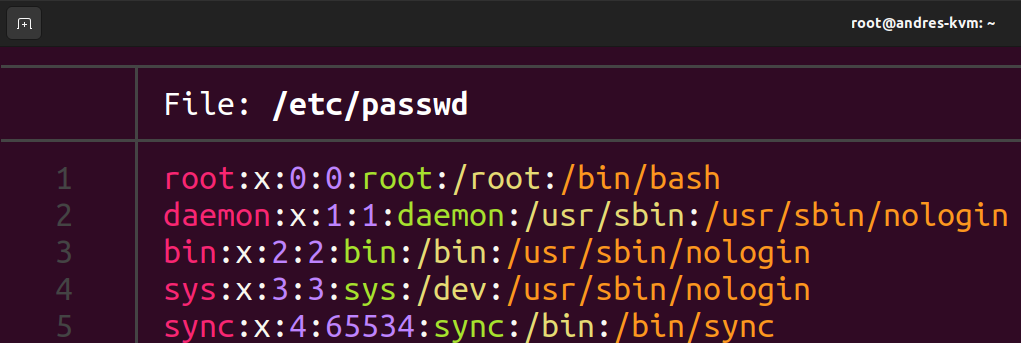
\includegraphics[width=\textwidth]{imagenes/passwdfile.png}
%\end{figure}

\phantomsection
\addcontentsline{toc}{section}{Ejercicio 1}
\section*{Ejercicio 1}

Voy a crear una partición con el sistema de archivos FAT32 (debido a problemas con Autopsy que me surgieron en los siguientes ejercicios) en el pendrive. Ahora a modo de realismo, voy a copiar las imágenes usadas durante estas prácticas y un archivo dentro de la carpeta ``mis trabajos'' denominado ``amenaza.txt'' con una frase que amenace.

%Foto de la carpeta con archivos y del archivo amenaza
\begin{figure}[H]
    \centering
    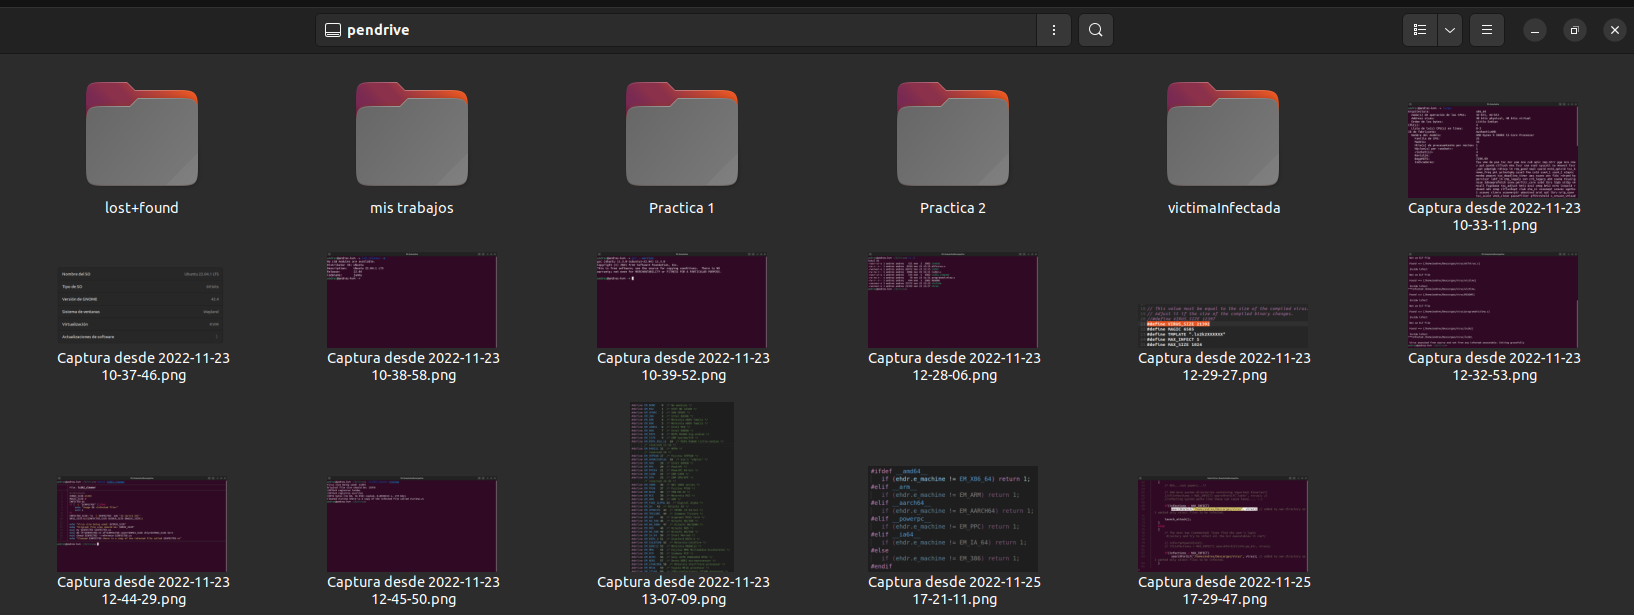
\includegraphics[width=\textwidth]{imagenes/Captura desde 2022-12-02 17-34-22.png}
    \caption{Archivos que he copiado al pendrive.}
\end{figure}

\begin{figure}[H]
    \centering
    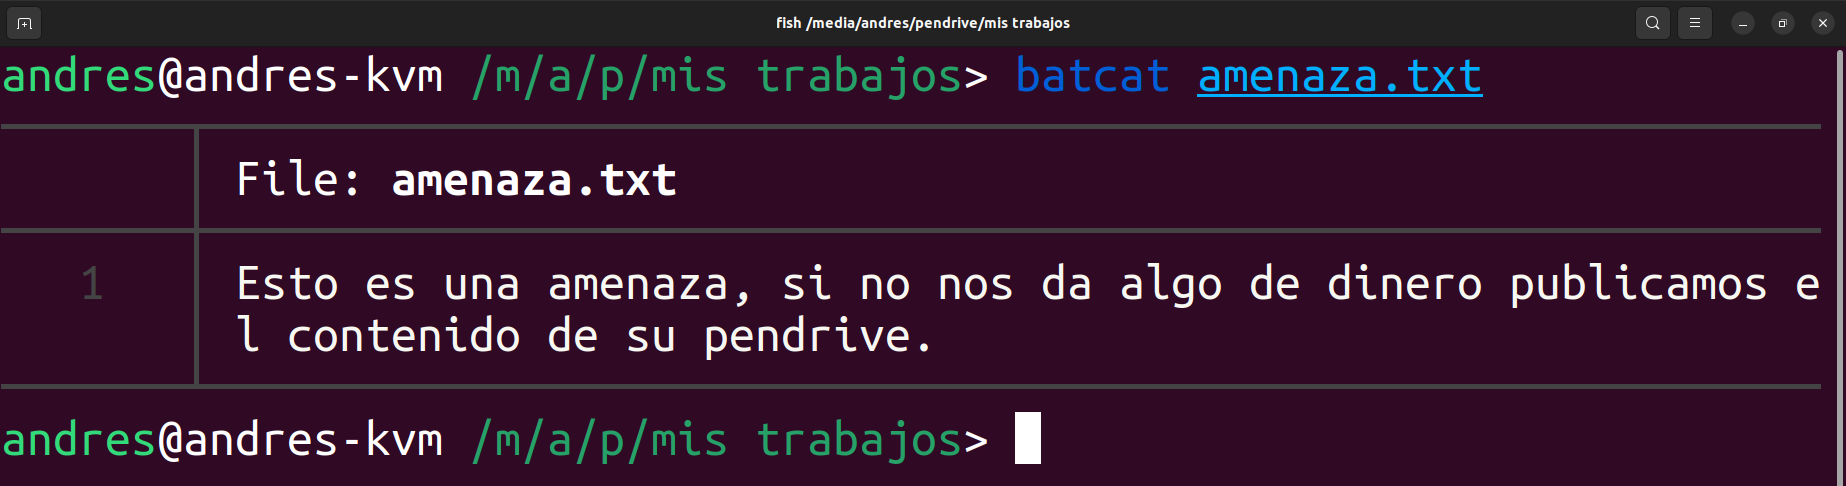
\includegraphics[width=\textwidth]{imagenes/Captura desde 2022-12-02 17-35-50.png}
    \caption{Contenido del archivo a eliminar del pendrive.}
\end{figure}

A continuación elimino ese archivo y desmonto el disco para suponer que he recibido el pendrive así y para que no pueda realizarle más modificaciones.

\bigskip

Ahora voy a seguir los pasos indicados en el guion de prácticas, por tanto, lo primero que hay que hacer es obtener la estructura interna de particiones con \verb|fdisk -l /dev/sdX > fdisk.disco1| siendo la X la letra asignada al disco, en mi caso es \verb|sda|. (se puede comprobar con la orden \verb|fdisk -l| o \verb|lsblk|).

%foto de la salida del comando
\begin{figure}[H]
    \centering
    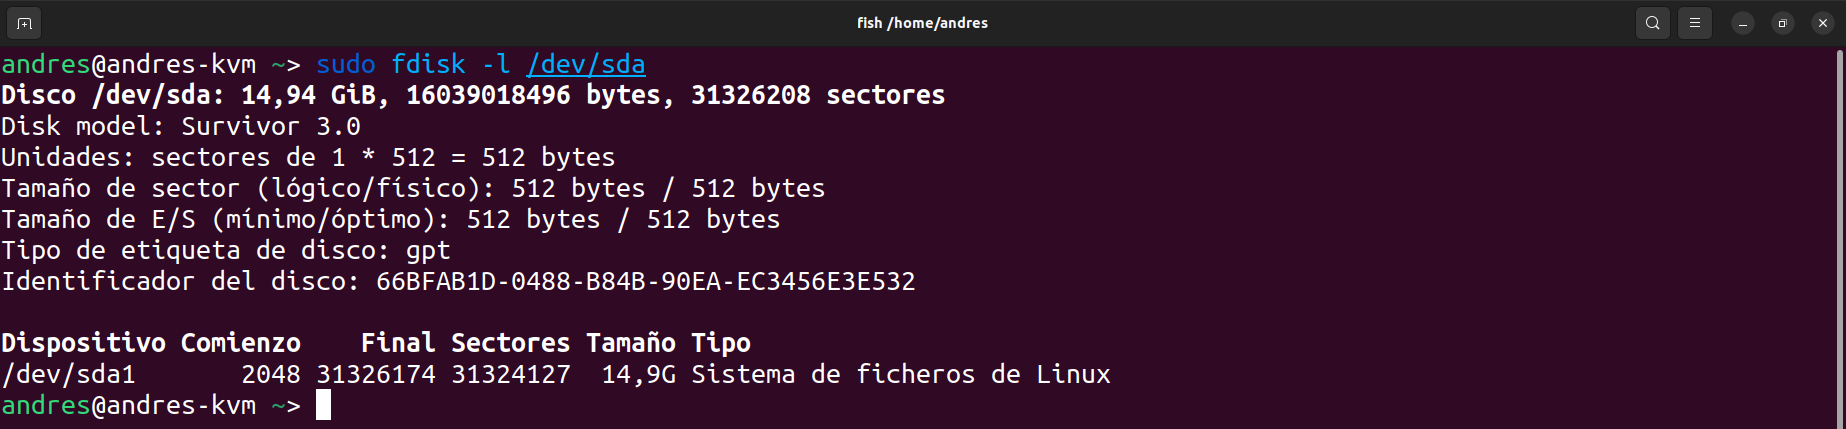
\includegraphics[width=\textwidth]{imagenes/Captura desde 2022-12-03 21-28-00.png}
    \caption{Salida del comando \texttt{fdisk}.}
\end{figure}

\newpage

Lo siguiente que hay que hacer es crear una imagen forense del disco para evitar invalidar el contenido del pendrive y trabajar de forma segura sobre una copia. Esto se realiza mediante la orden \verb|dd if=/dev/sda1 of=imagen.disco1 bs=512|.

%salida de dd
\begin{figure}[H]
    \centering
    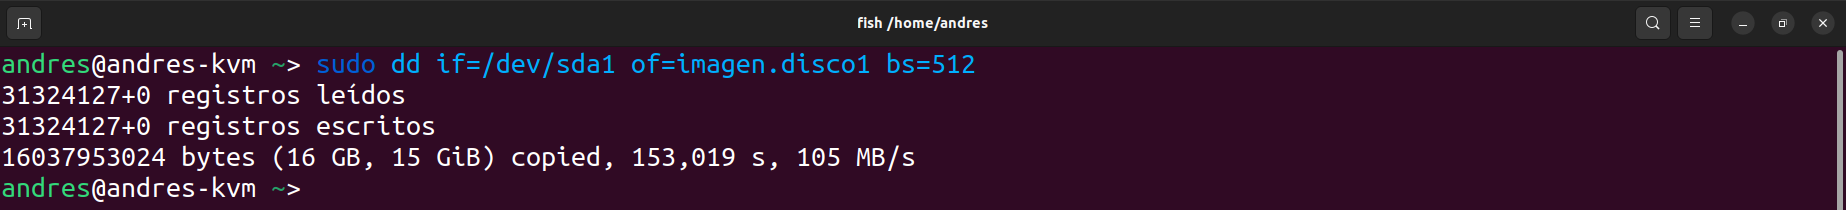
\includegraphics[width=\textwidth]{imagenes/Captura desde 2022-12-03 21-31-25.png}
    \caption{Salida de la copia de la partición del pendrive a un archivo.}
\end{figure}

Ahora es necesario poner la imagen del disco a solo lectura con \verb|chmod 444 imagen.disco1|. El siguiente paso, que es copiar la imagen a otro disco no es necesario, ya que se puede trabajar directamente sobre la imagen como explicaré a continuación. Ahora se debe montar la imagen con la orden \verb|mount imagen.disco1 /mnt -o noexec,loop|, y al hacer \verb|lsblk -f| se puede ver que está montado correctamente.

%foto de la salida de lsblk
\begin{figure}[H]
    \centering
    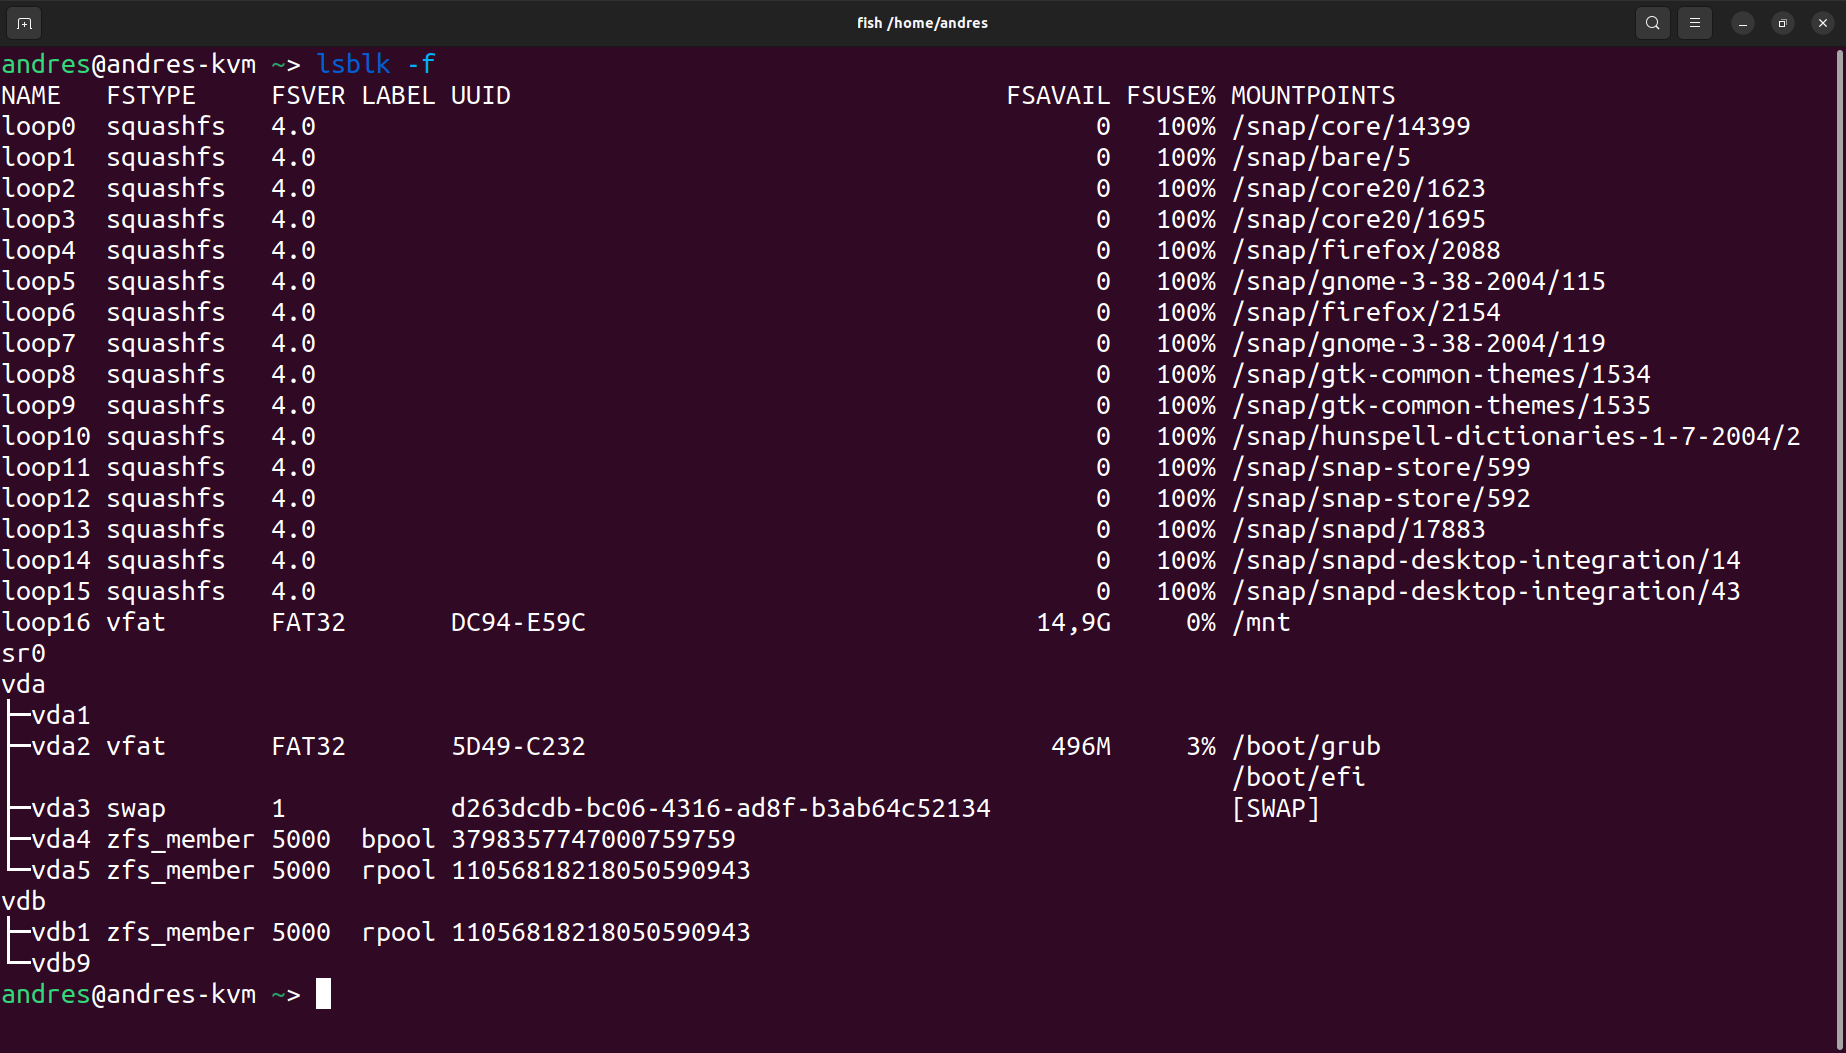
\includegraphics[width=\textwidth]{imagenes/Captura desde 2022-12-03 21-32-34.png}
    \caption{Se puede ver que el nombre que tiene es \texttt{loop16} y que se ha montado correctamente en el punto de montaje indicado.}
\end{figure}

También es necesario verificar la integridad de los datos del pendrive antes y después de completar el análisis, para ello se usa la orden \verb|sha1sum /dev/sda1 > SHA.disco1|.

%foto de sha1sum
\begin{figure}[H]
    \centering
    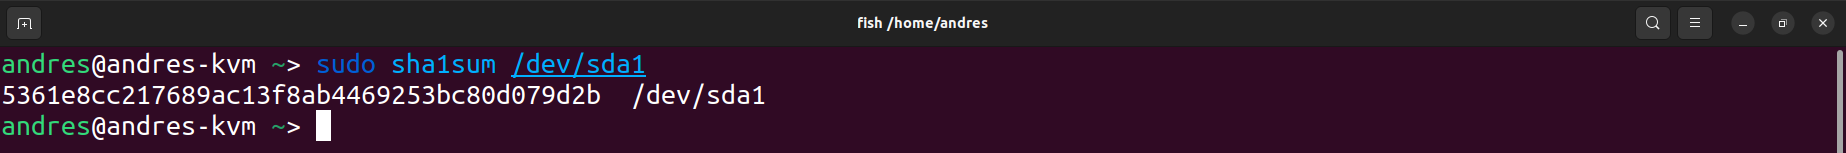
\includegraphics[width=\textwidth]{imagenes/Captura desde 2022-12-03 21-36-15.png}
    \caption{Salida de la orden \texttt{sha1sum}.}
\end{figure}

\newpage

Y ahora, voy a realizar lo mismo, pero sobre cada archivo. En este caso se debe hacer sobre la imagen porque al montar el pendrive puede darse el caso de que el hash cambie. Para ello, desde la raíz de la imagen montada, se debe hacer con la orden siguiente: 

\verb|find . -type f -exec sha1sum {} \; > SHA.listaArchivos|.

%salida del comando con bat
\begin{figure}[H]
    \centering
    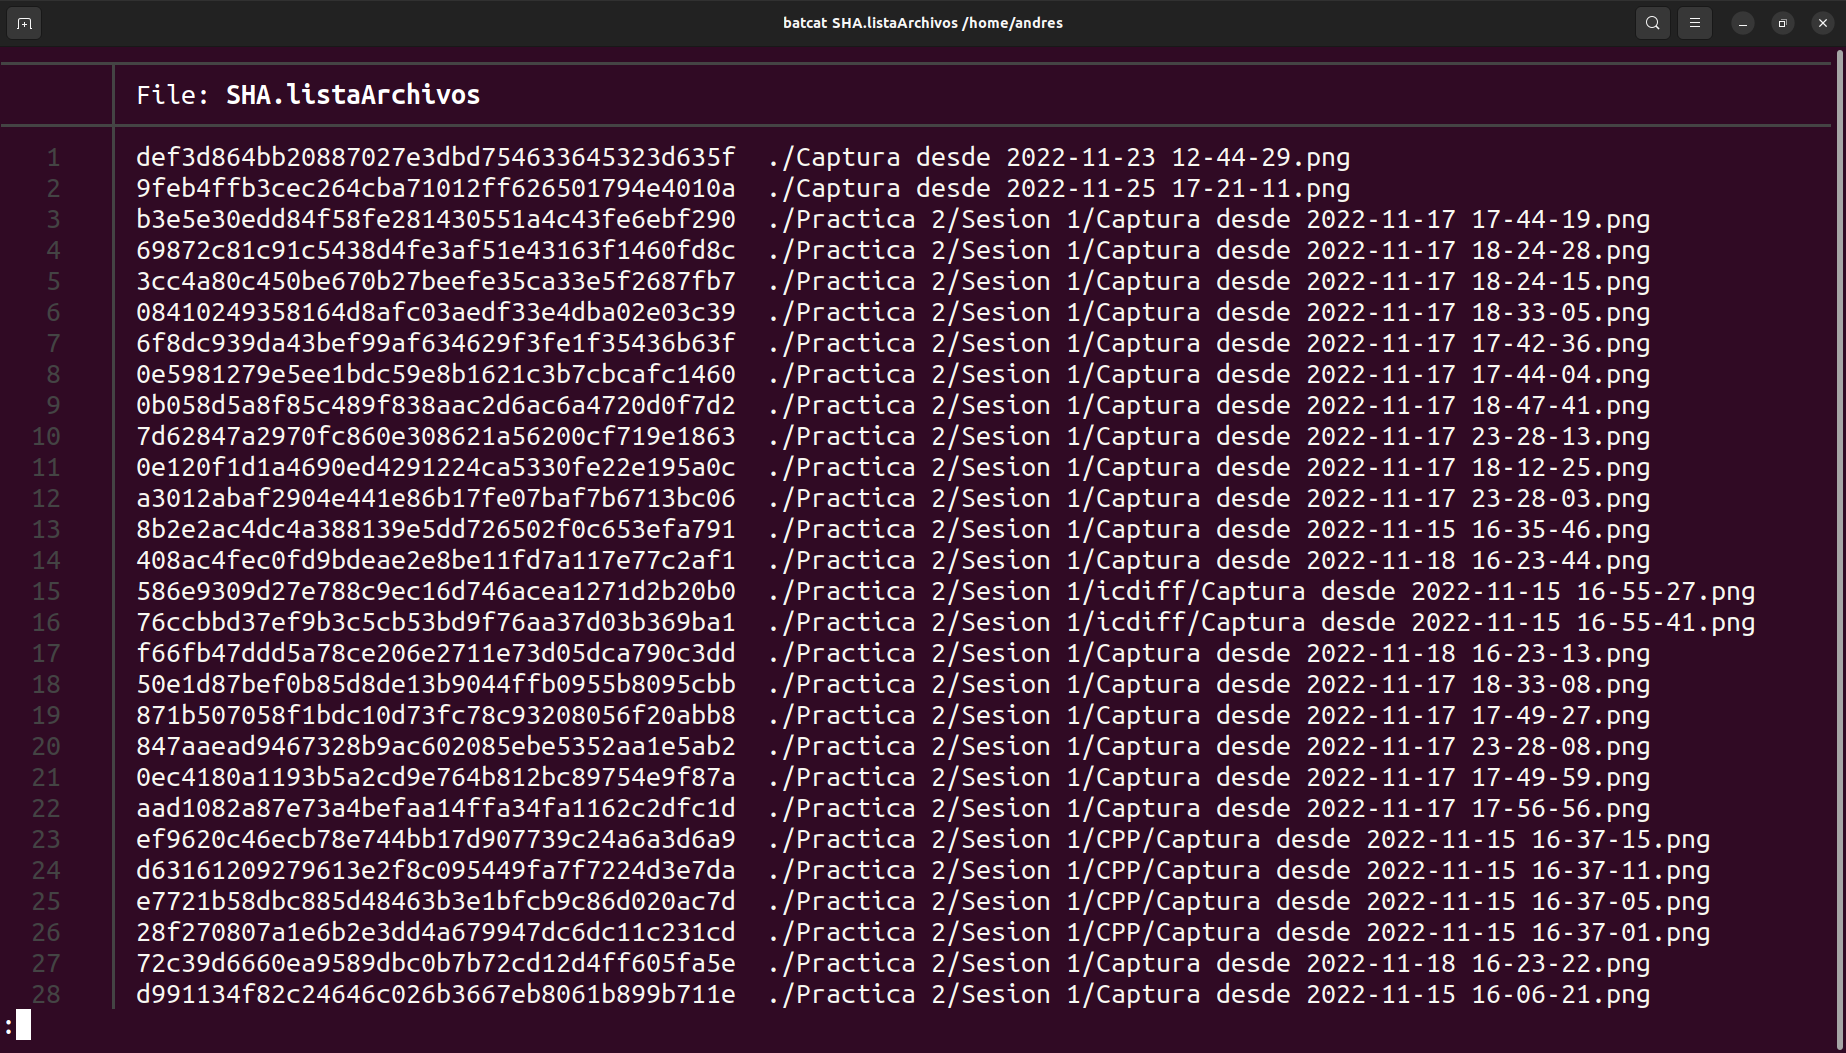
\includegraphics[width=\textwidth]{imagenes/Captura desde 2022-12-02 18-41-07.png}
    \caption{Hash de cada archivo de la imagen.}
\end{figure}

Y se puede realizar la verificación con la orden \verb|sha1sum -c ~/SHA.listaArchivos| (se debe estar dentro de la raíz de la imagen)

%salida del comando.
\begin{figure}[H]
    \centering
    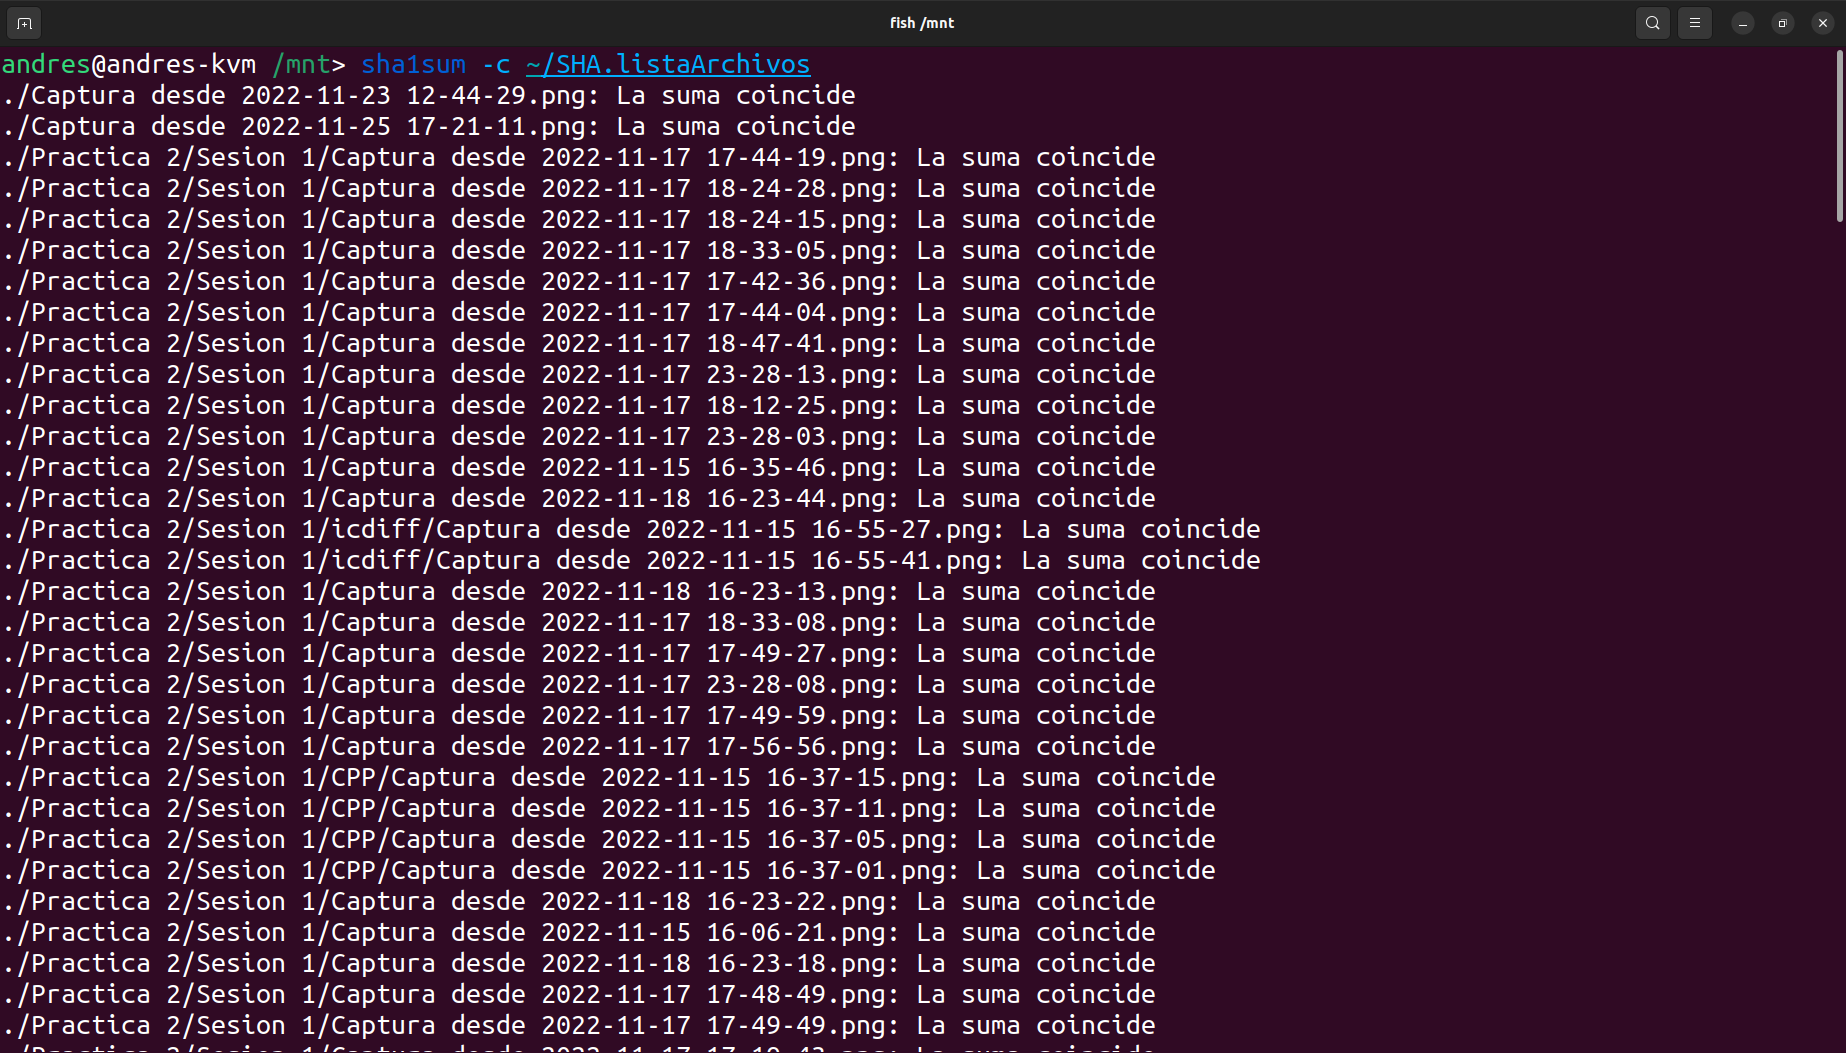
\includegraphics[width=\textwidth]{imagenes/Captura desde 2022-12-02 18-43-28.png}
    \caption{Fragmento de la comprobación de los hashes.}
\end{figure}

\newpage

Ahora se puede proceder con seguridad a encontrar el archivo eliminado anteriormente. Para ello, es necesario crear un fichero con las palabras claves más probables que se encuentren. El fichero tiene la siguiente forma:

%slaida
\begin{figure}[H]
    \centering
    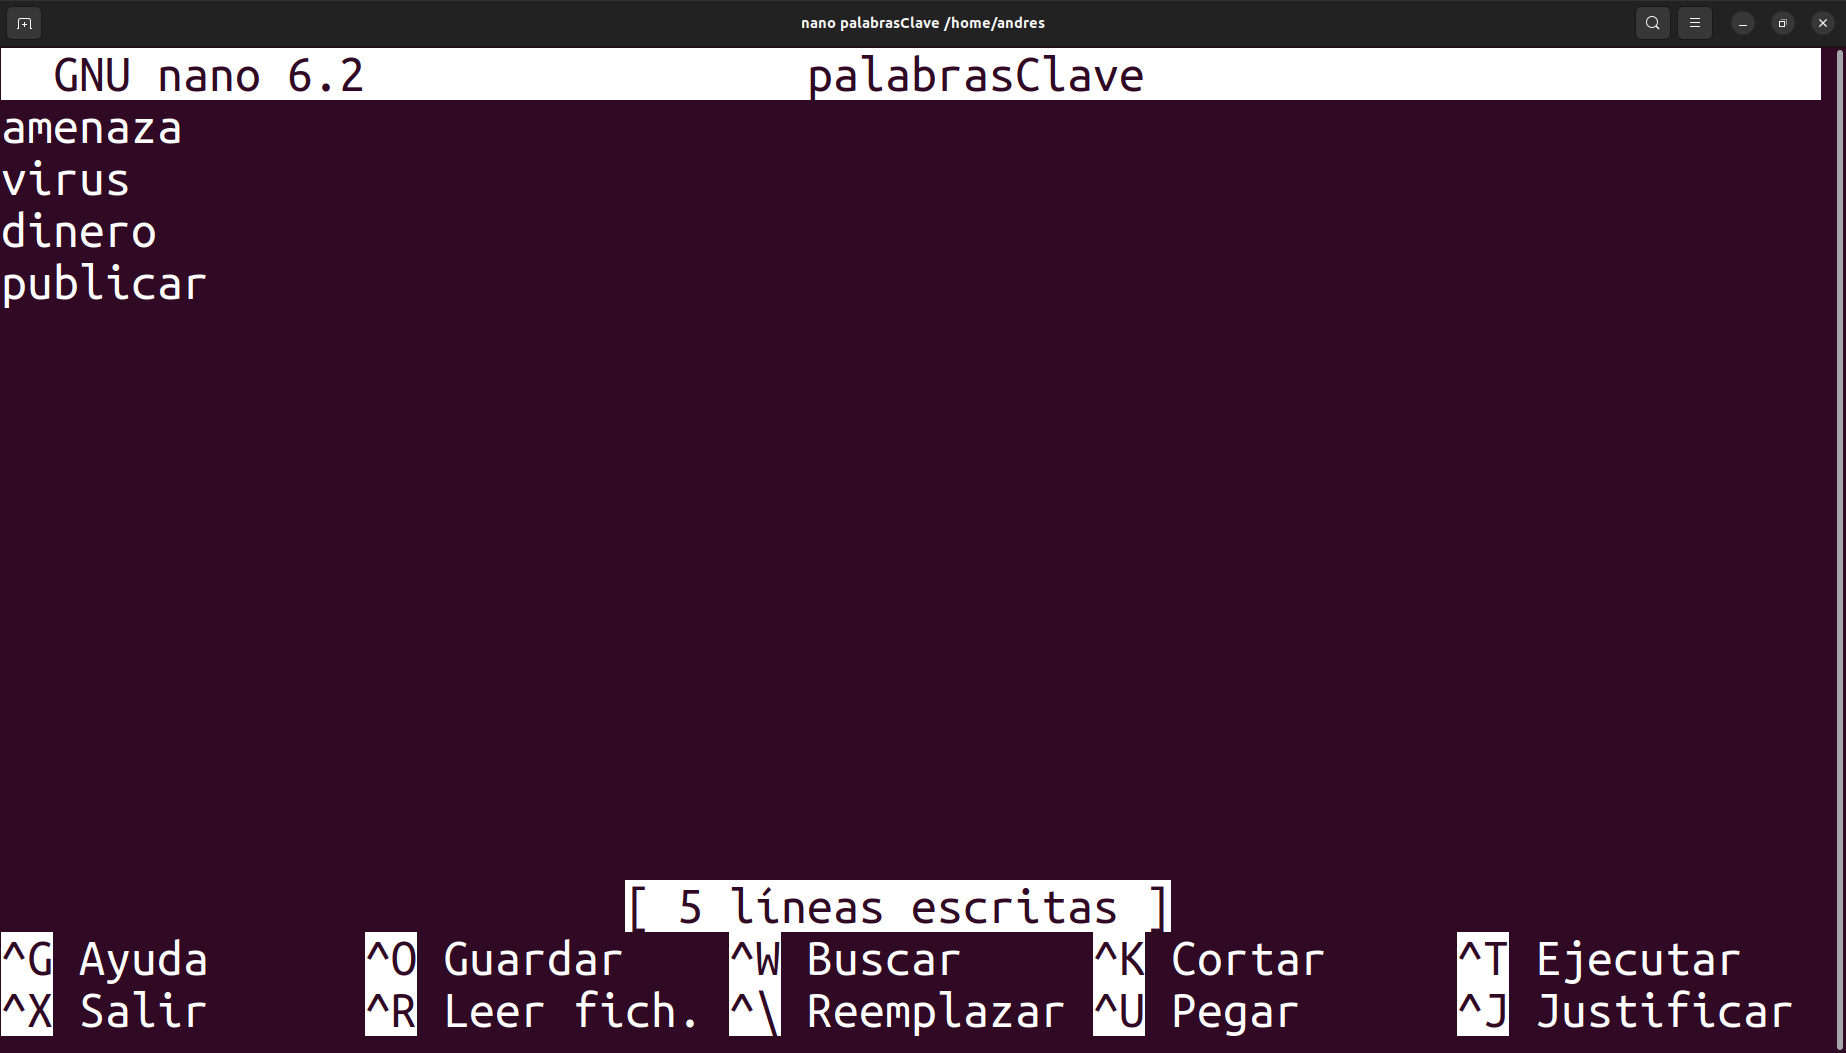
\includegraphics[width=\textwidth]{imagenes/Captura desde 2022-12-02 18-52-07.png}
    \caption{Diccionario de palabras clave a buscar en la imagen.}
\end{figure}

Ahora con la orden \verb|grep -aibf palabrasClave imagen.disco1 > aciertos.txt| se puede realizar la búsqueda en la imagen:

%salida en aciertos.txt
\begin{figure}[H]
    \centering
    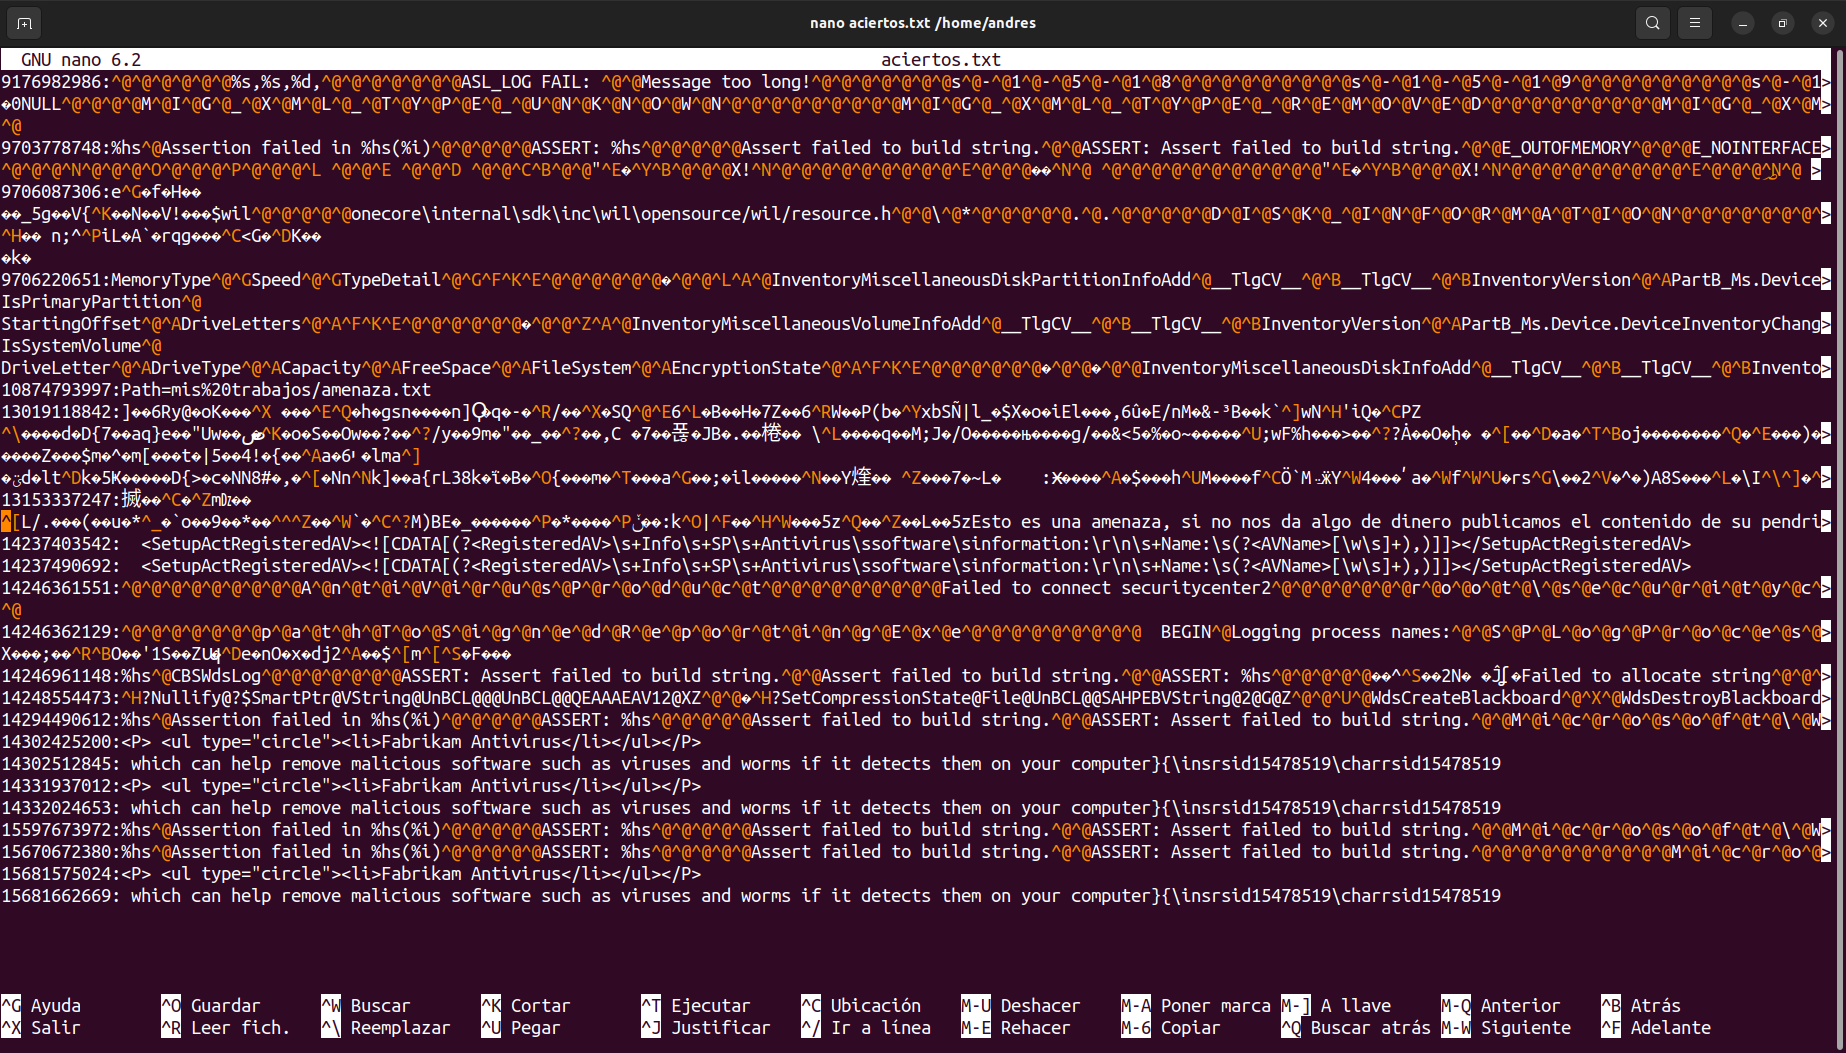
\includegraphics[width=\textwidth]{imagenes/Captura desde 2022-12-03 21-38-57.png}
    \caption{En la dirección 13153337247 hay algo sospechoso.}
\end{figure}
Como se puede ver, aparece la frase ``Esto es una amenaza, si no nos da algo de dinero publicamos el contenido de su pendri...'', indicando que ha habido una amenaza.

\newpage

Por último, para asegurarse, se puede usar el comando \texttt{xxd -s 299892684 imagen.disco1 | less} para verlo en la propia imagen:

%salida del comando
\begin{figure}[H]
    \centering
    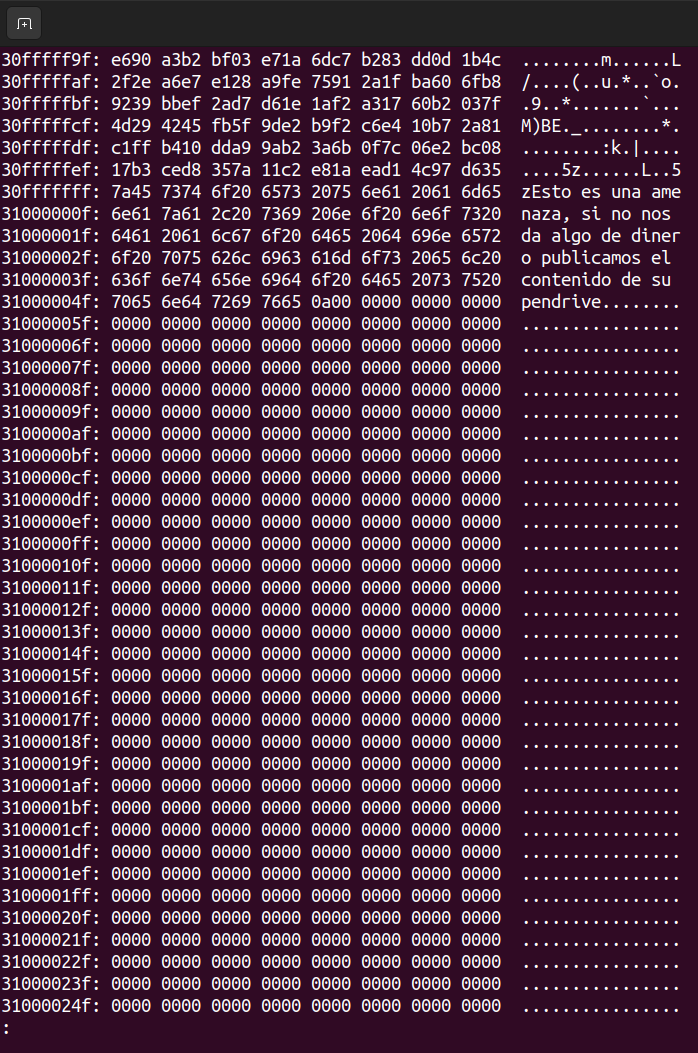
\includegraphics[width=0.6\textwidth]{imagenes/Captura desde 2022-12-03 21-39-24.png}
    \caption{Se puede ver a la derecha que aparece el contenido del archivo eliminado.}
\end{figure}

Y efectivamente, aquí también aparece indicando de que ha habido una amenaza que se ha eliminado.

\newpage

\phantomsection
\addcontentsline{toc}{section}{Ejercicio 2}
\section*{Ejercicio 2}

En esta parte es necesario utilizar la herramienta ``GuyMager'' para obtener una imagen forense del mismo pendrive. Por tanto, se descarga el programa mediante \verb|apt| y se abre.

%foto de inicio.
\begin{figure}[H]
    \centering
    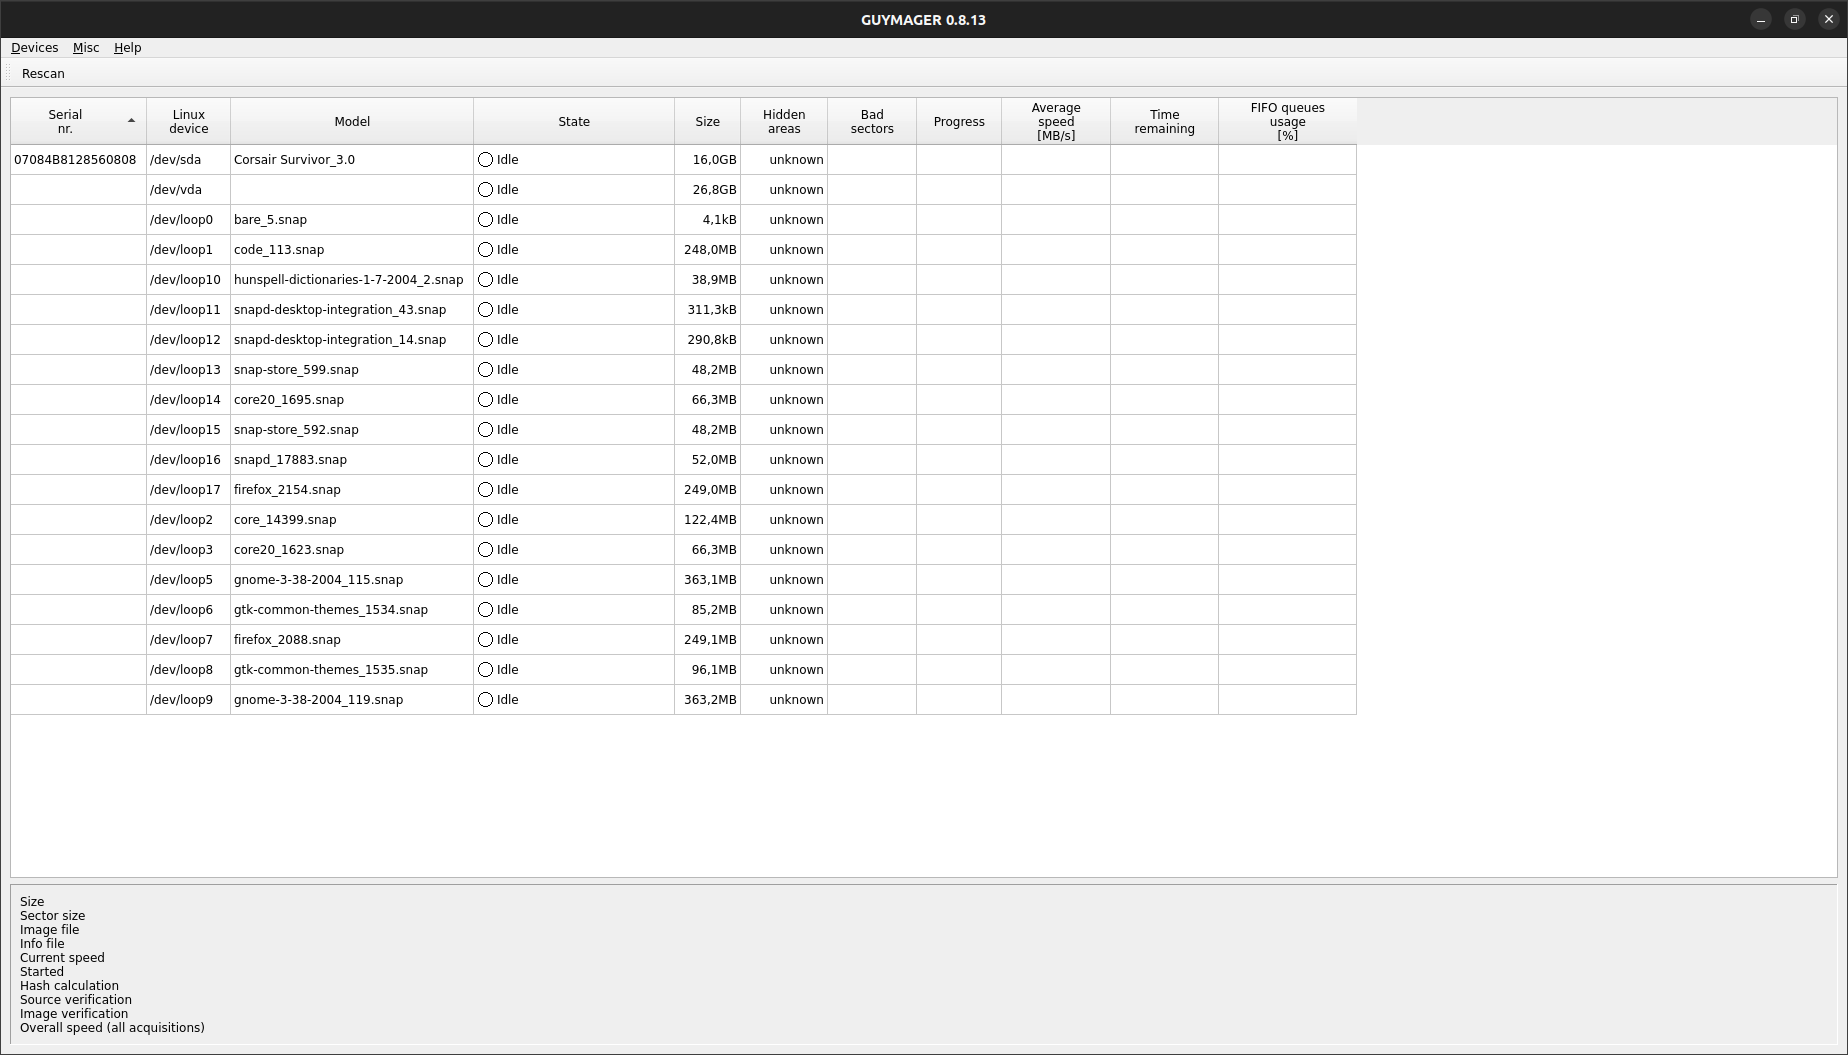
\includegraphics[width=\textwidth]{imagenes/Captura desde 2022-12-02 19-33-30.png}
    \caption{Ventana inicial del programa.}
\end{figure}

Y se pulsa con clic derecho en el dispositivo que se quiera realizar la imagen, en mi caso \verb|/dev/sda|, y le damos a ``Acquire image''.

%ventana nueva
\begin{figure}[H]
    \centering
    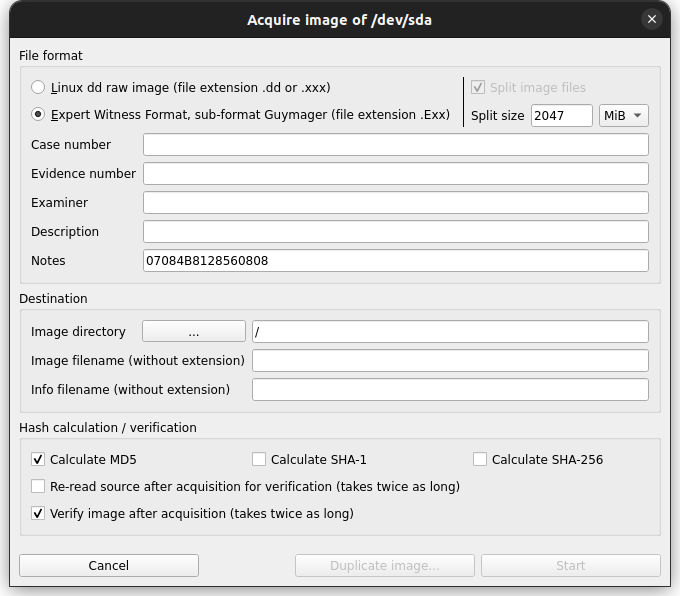
\includegraphics[width=0.7\textwidth]{imagenes/Captura desde 2022-12-02 19-33-37.png}
    \caption{Ventana para rellenar datos sobre la imagen.}
\end{figure}

\newpage

Y ahora simplemente rellenamos los campos que se piden y al final quedan así:

%foto de esto relleno
\begin{figure}[H]
    \centering
    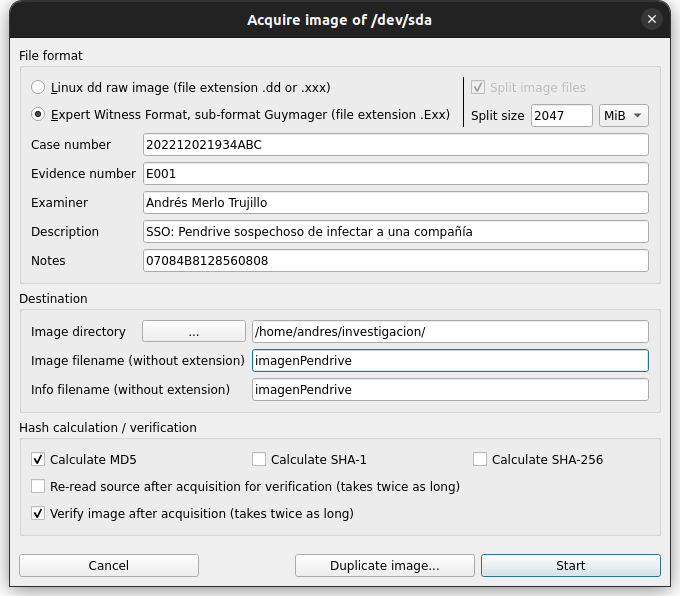
\includegraphics[width=0.7\textwidth]{imagenes/Captura desde 2022-12-02 19-36-04.png}
    \caption{Campos rellenados de la ventana anterior.}
\end{figure}

Por último, es necesario darle a ``Start'' para que comience el proceso.

%foto del progreso
\begin{figure}[H]
    \centering
    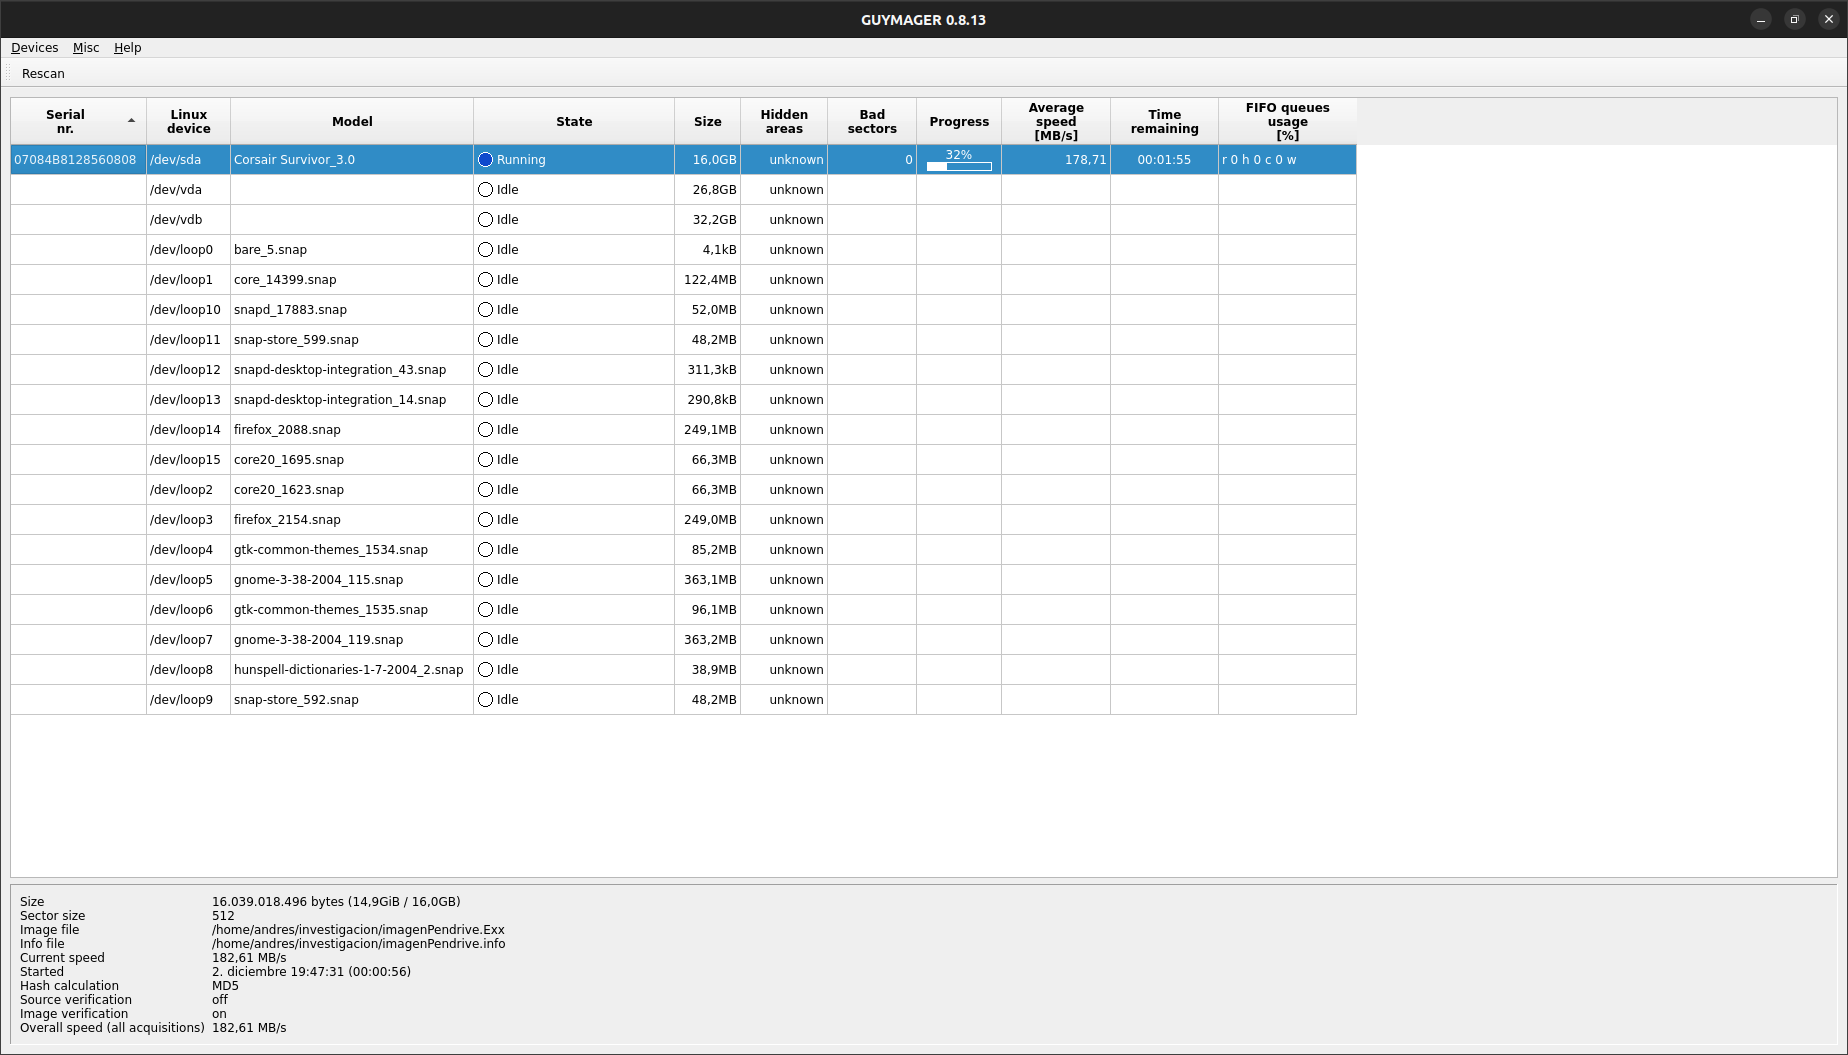
\includegraphics[width=\textwidth]{imagenes/Captura desde 2022-12-02 19-48-29.png}
    \caption{Progreso de creación de imagen forense.}
\end{figure}

\newpage

Al finalizar, se puede ver que ha generado varios trozos de la imagen del pendrive.

%foto
\begin{figure}[H]
    \centering
    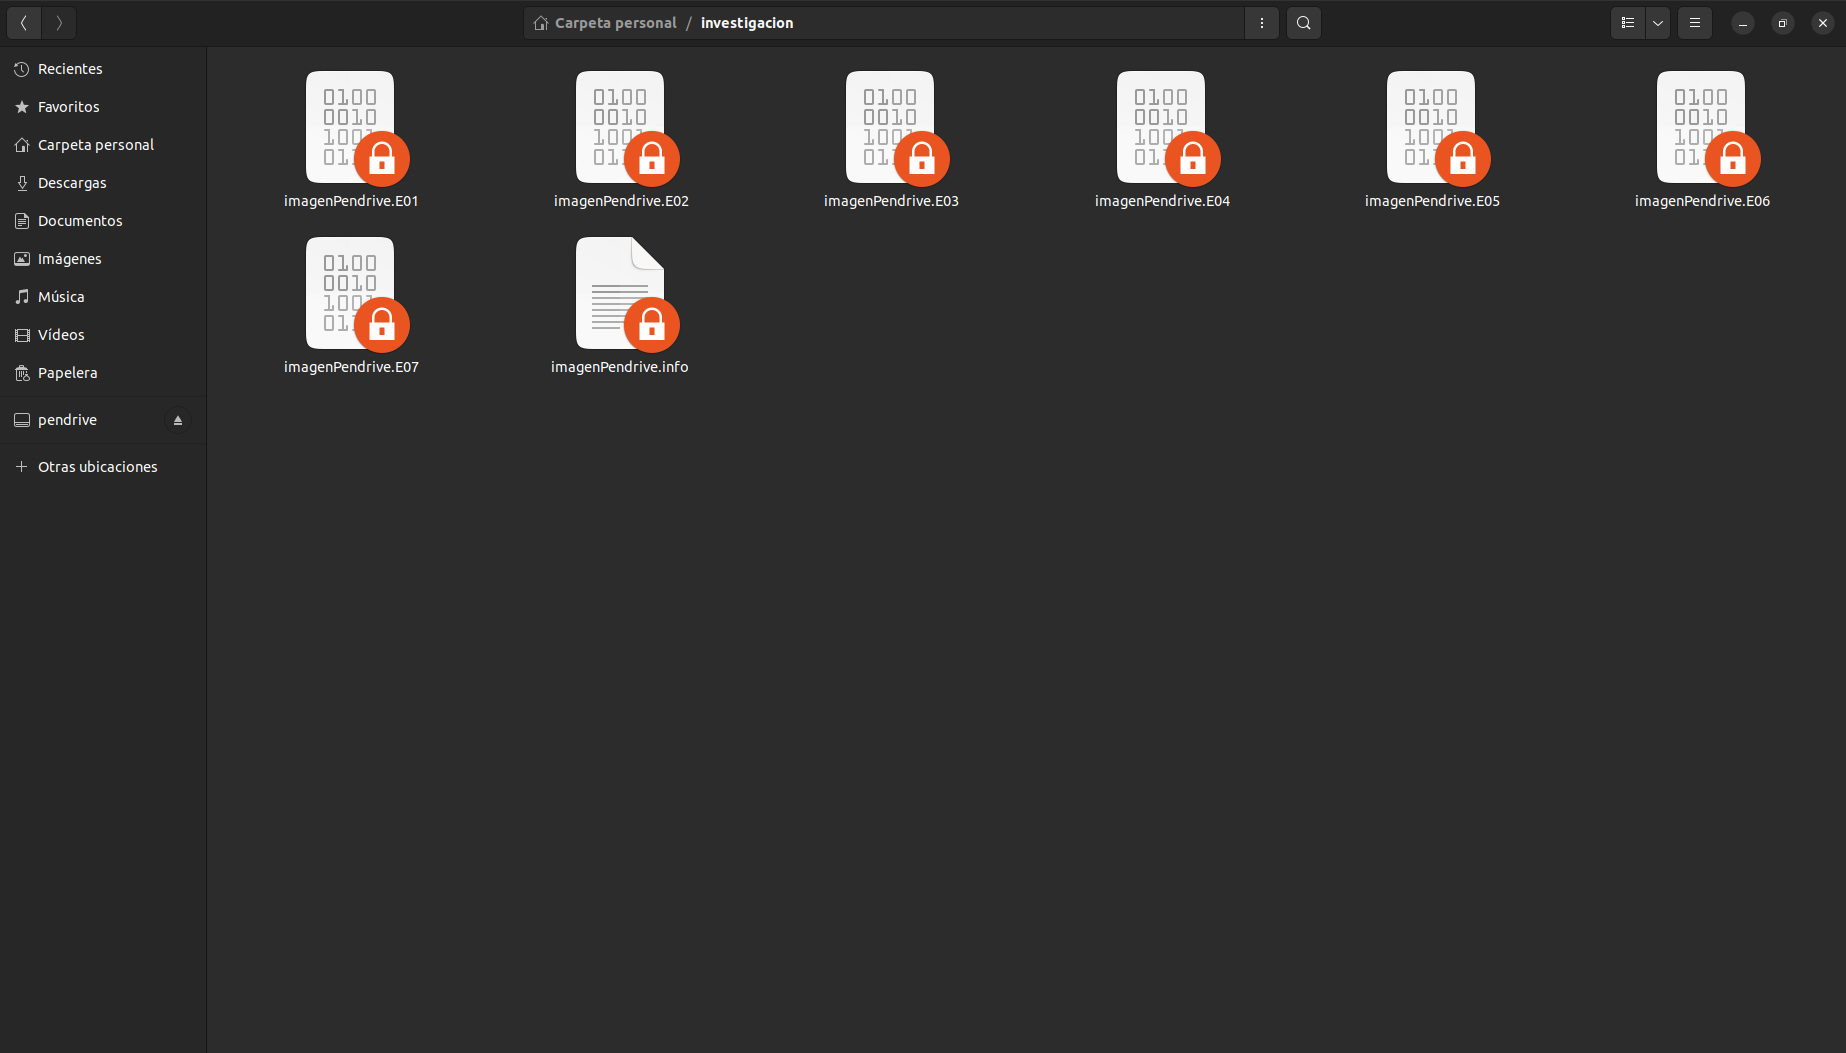
\includegraphics[width=\textwidth]{imagenes/Captura desde 2022-12-02 19-50-53.png}
    \caption{Archivos generados por el programa.}
\end{figure}

\phantomsection
\addcontentsline{toc}{section}{Ejercicio 3}
\section*{Ejercicio 3}

\textbf{NOTA: }La versión de Autopsy para Linux con la interfaz web no era capaz de detectar las particiones de la imagen creada con la herramienta del ejercicio anterior, por lo que he decidido usar la última versión de Autopsy que sí la detecta.

\phantomsection
\addcontentsline{toc}{subsection}{Apartado A}
\subsection*{Apartado A}

Cuando se ejecuta Autopsy aparece la siguiente pantalla:

%foto pantalla
\begin{figure}[H]
    \centering
    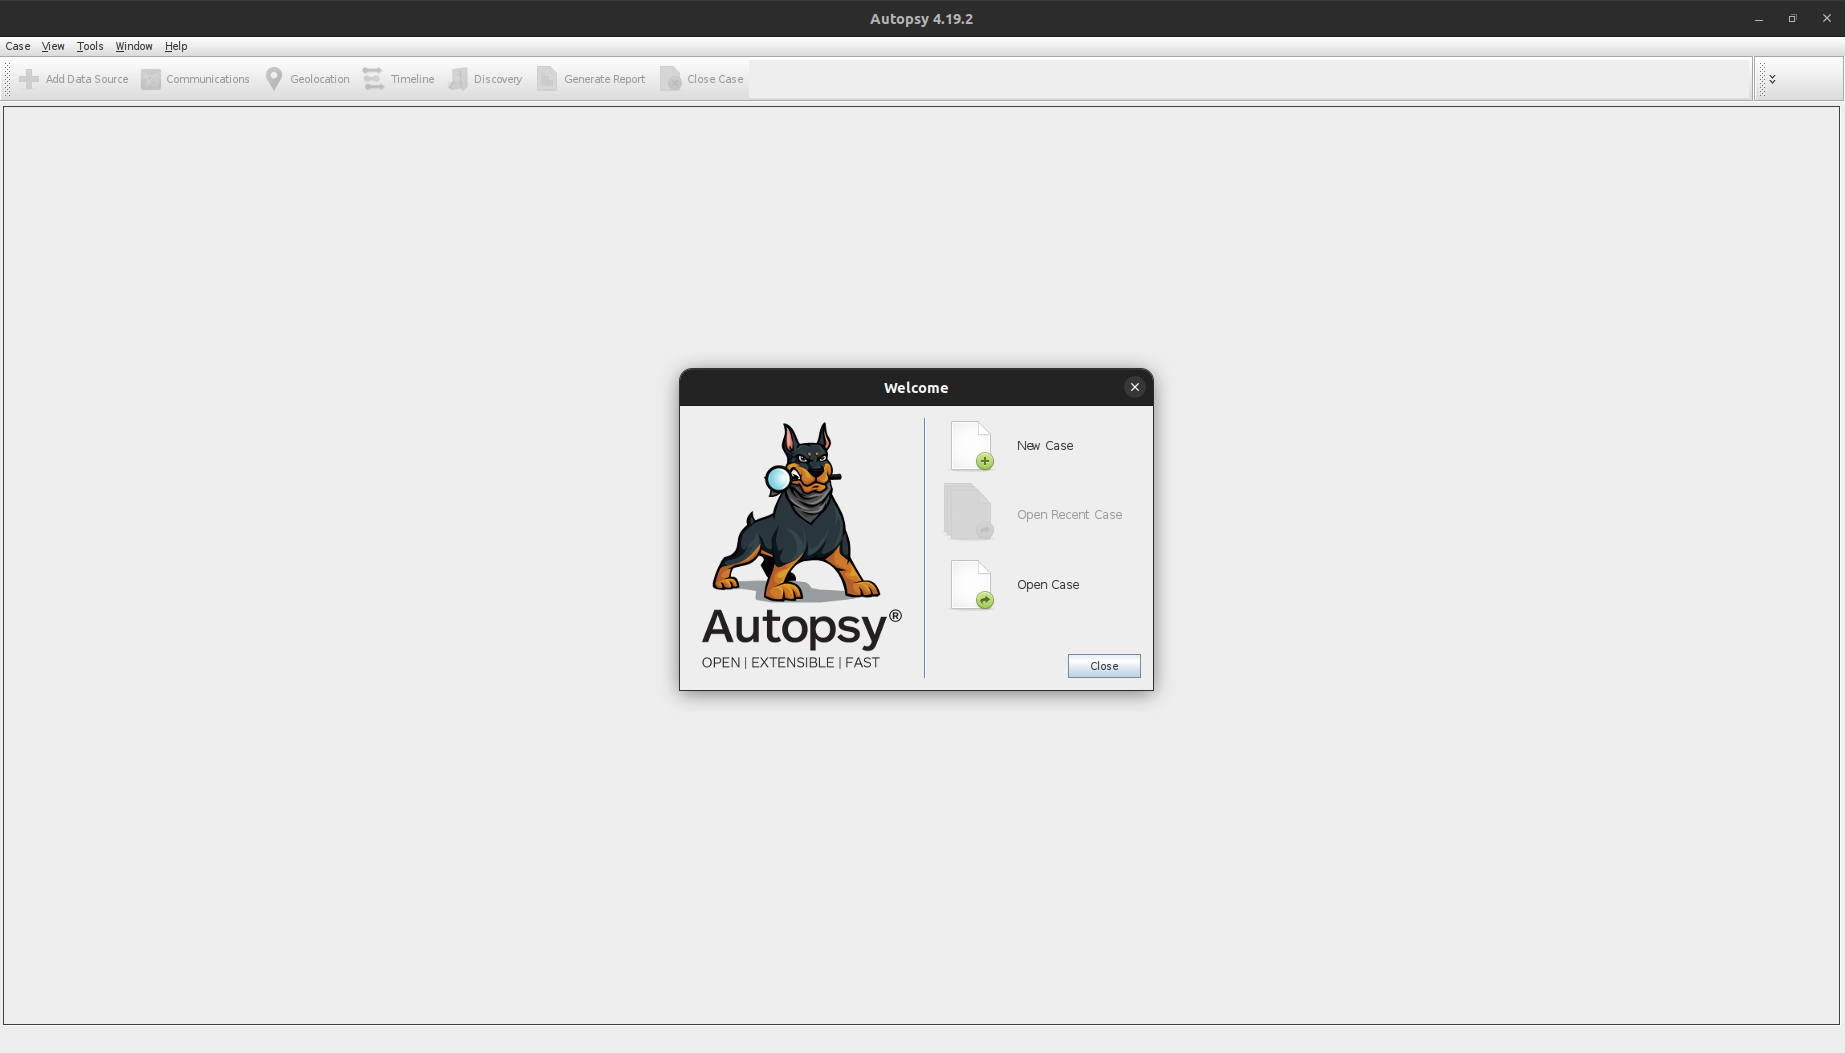
\includegraphics[width=\textwidth]{imagenes/Captura desde 2022-12-03 21-22-16.png}
\end{figure}

\newpage

Ahora le damos a ``New Case'' y se le elige un nombre, la ubicación, el número de caso, algunos datos del examinador:

%fotos rellenas
\begin{figure}[H]
    \centering
    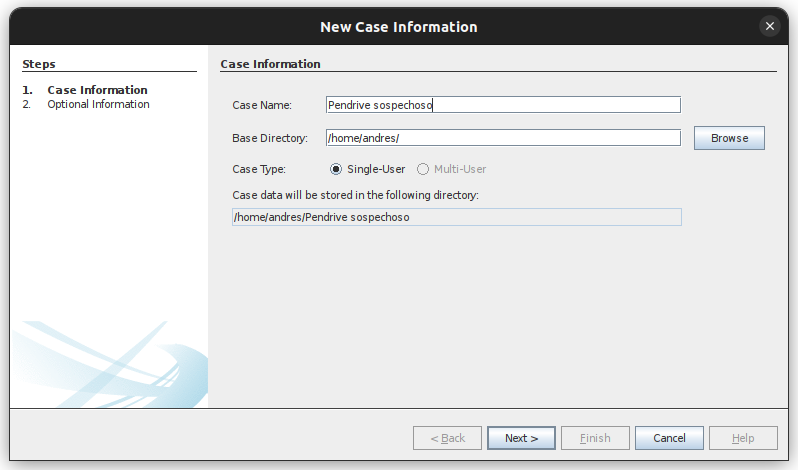
\includegraphics[width=\textwidth]{imagenes/Captura desde 2022-12-03 21-42-29.png}
    \caption{Primera ventana para rellenar datos sobre el caso.}
\end{figure}

\begin{figure}[H]
    \centering
    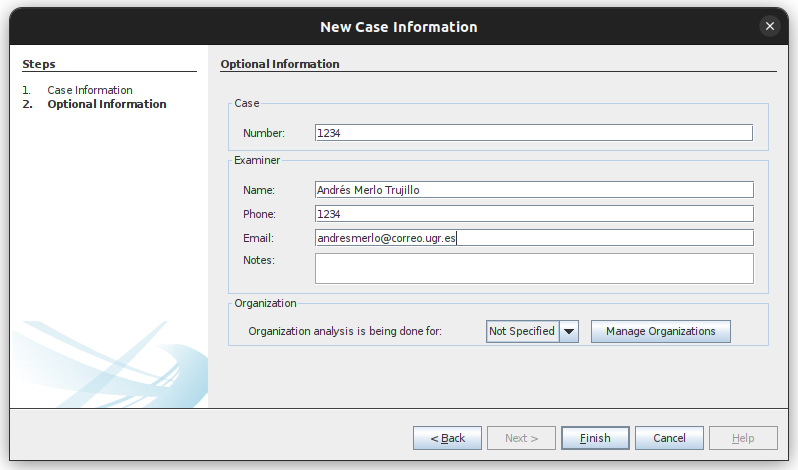
\includegraphics[width=\textwidth]{imagenes/Captura desde 2022-12-03 21-43-15.png}
    \caption{Segunda venta para rellenar datos sobre el caso.}
\end{figure}

\newpage

Al darle a Finish, aparece otra ventana en la que se pide añadir una fuente de datos, en este caso la imagen creada, para ello se elige ``Disk Image or VM File'' y se elige el primer fragmento de la imagen:

%fotos rellenas
\begin{figure}[H]
    \centering
    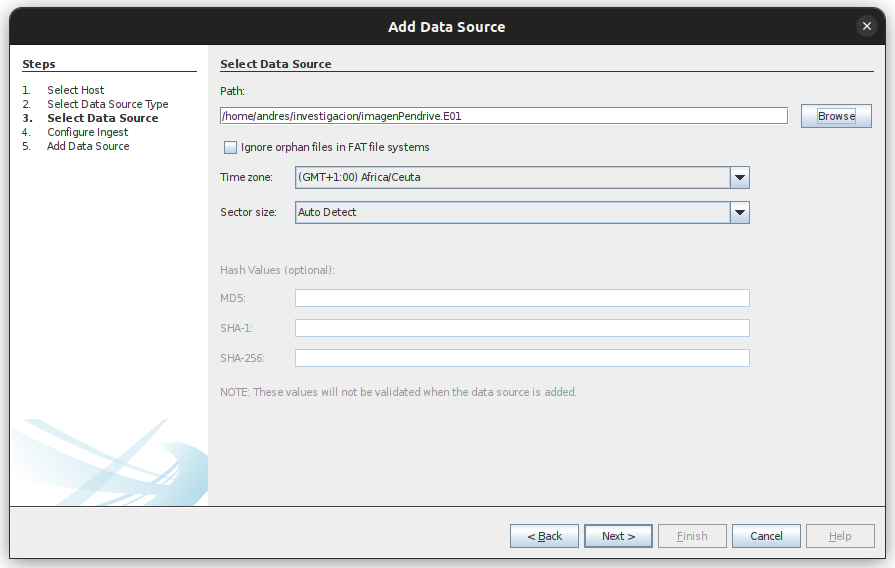
\includegraphics[width=\textwidth]{imagenes/Captura desde 2022-12-03 21-45-13.png}
    \caption{Selección de la imagen creada con GuyMager.}
\end{figure}

Tras que el programa procese la imagen, aparece el siguiente panel:

%foto panel
\begin{figure}[H]
    \centering
    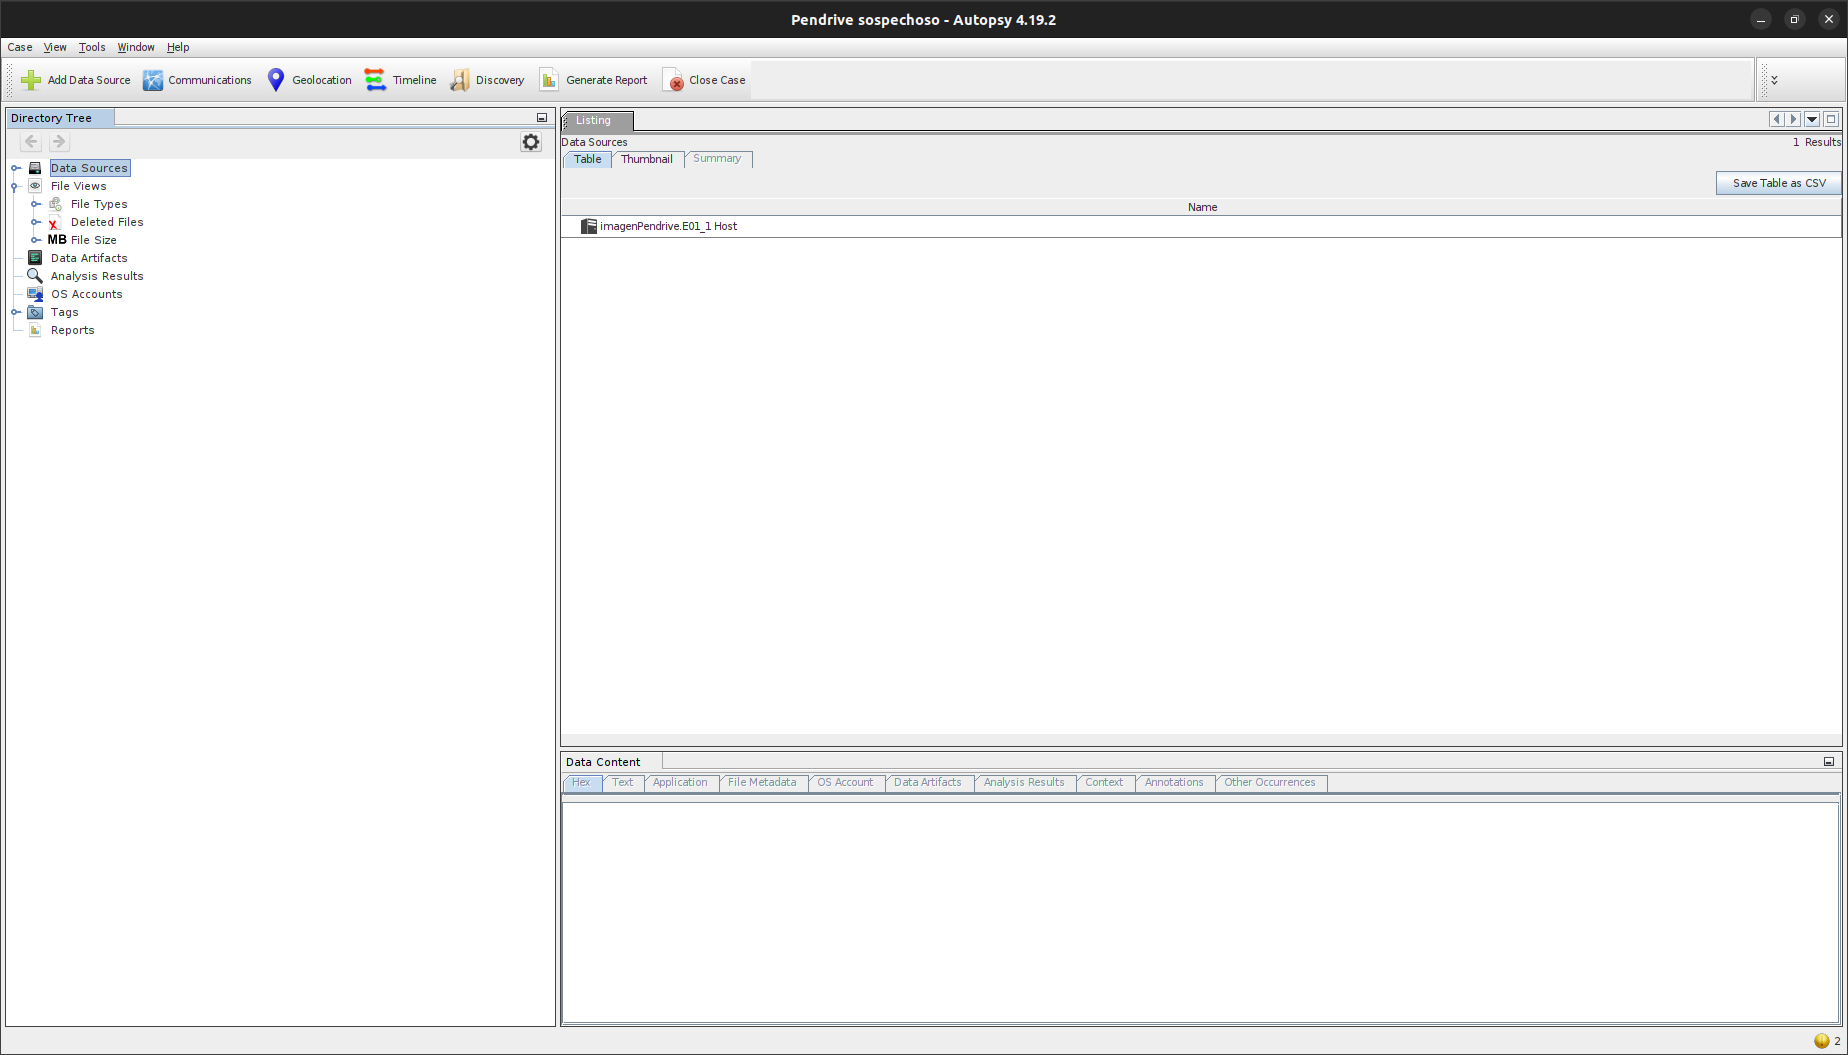
\includegraphics[width=\textwidth]{imagenes/Captura desde 2022-12-03 21-46-02.png}
    \caption{Pantalla principal de Autopsy.}
\end{figure}

\newpage

Y ahora vamos a Data Sources $\rightarrow$ imagenPendrive.E01\_1 Host $\rightarrow$ imagenPendrive.E01 $\rightarrow$ vol4.

%foto salida
\begin{figure}[H]
    \centering
    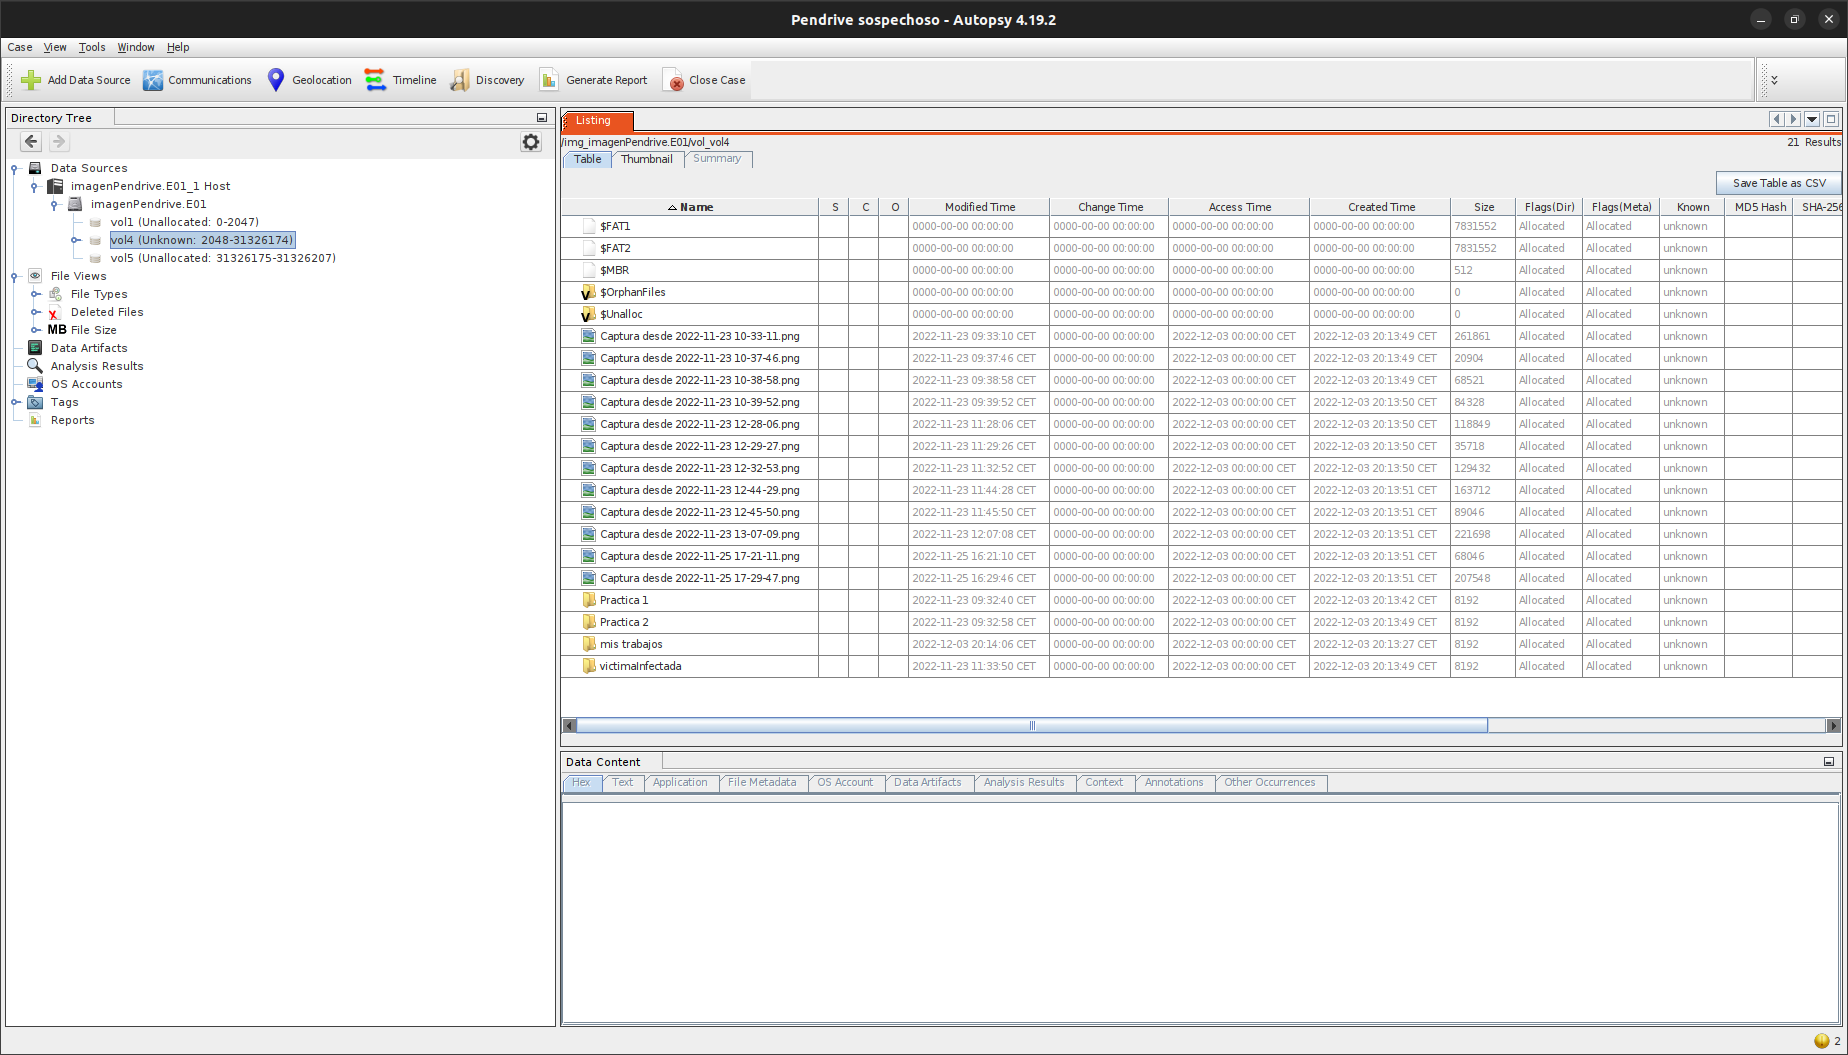
\includegraphics[width=\textwidth]{imagenes/Captura desde 2022-12-03 21-47-44.png}
    \caption{Archivos que contiene la imagen.}
\end{figure}

Como se puede ver, hay 3 particiones que hacían que versiones antiguas de Autopsy (con interfaz web) no pudiesen detectar el sistema de archivos correctamente y solo funcionasen en modo raw.

\bigskip

Ahora bien, hay dos opciones de ver archivos eliminados: la primera es yendo a la ubicación donde estaba el archivo, y la segunda es dándole al botón del panel de la izquierda ``Deleted Files''.

%foto de deleted files y el otro
\begin{figure}[H]
    \centering
    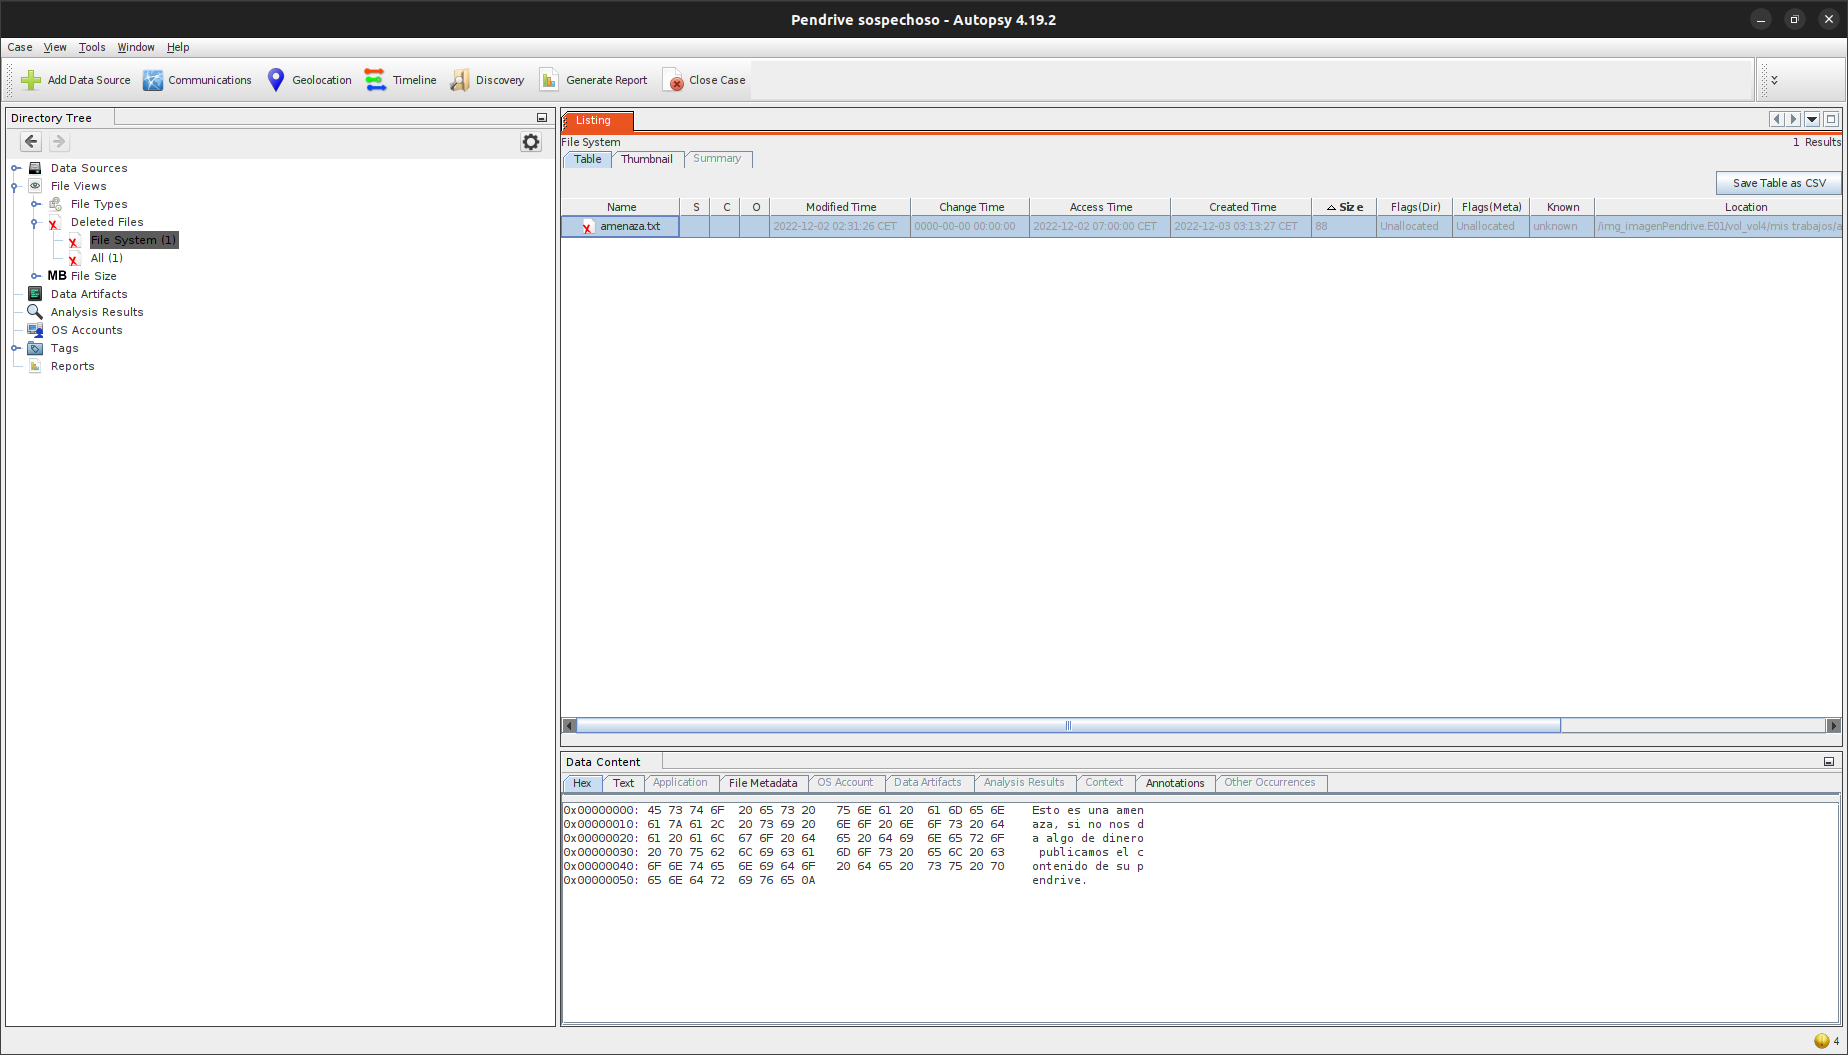
\includegraphics[width=\textwidth]{imagenes/Captura desde 2022-12-03 21-52-53.png}
    \caption{Archivo encontrado en ``Deleted Files''.}
\end{figure}

\begin{figure}[H]
    \centering
    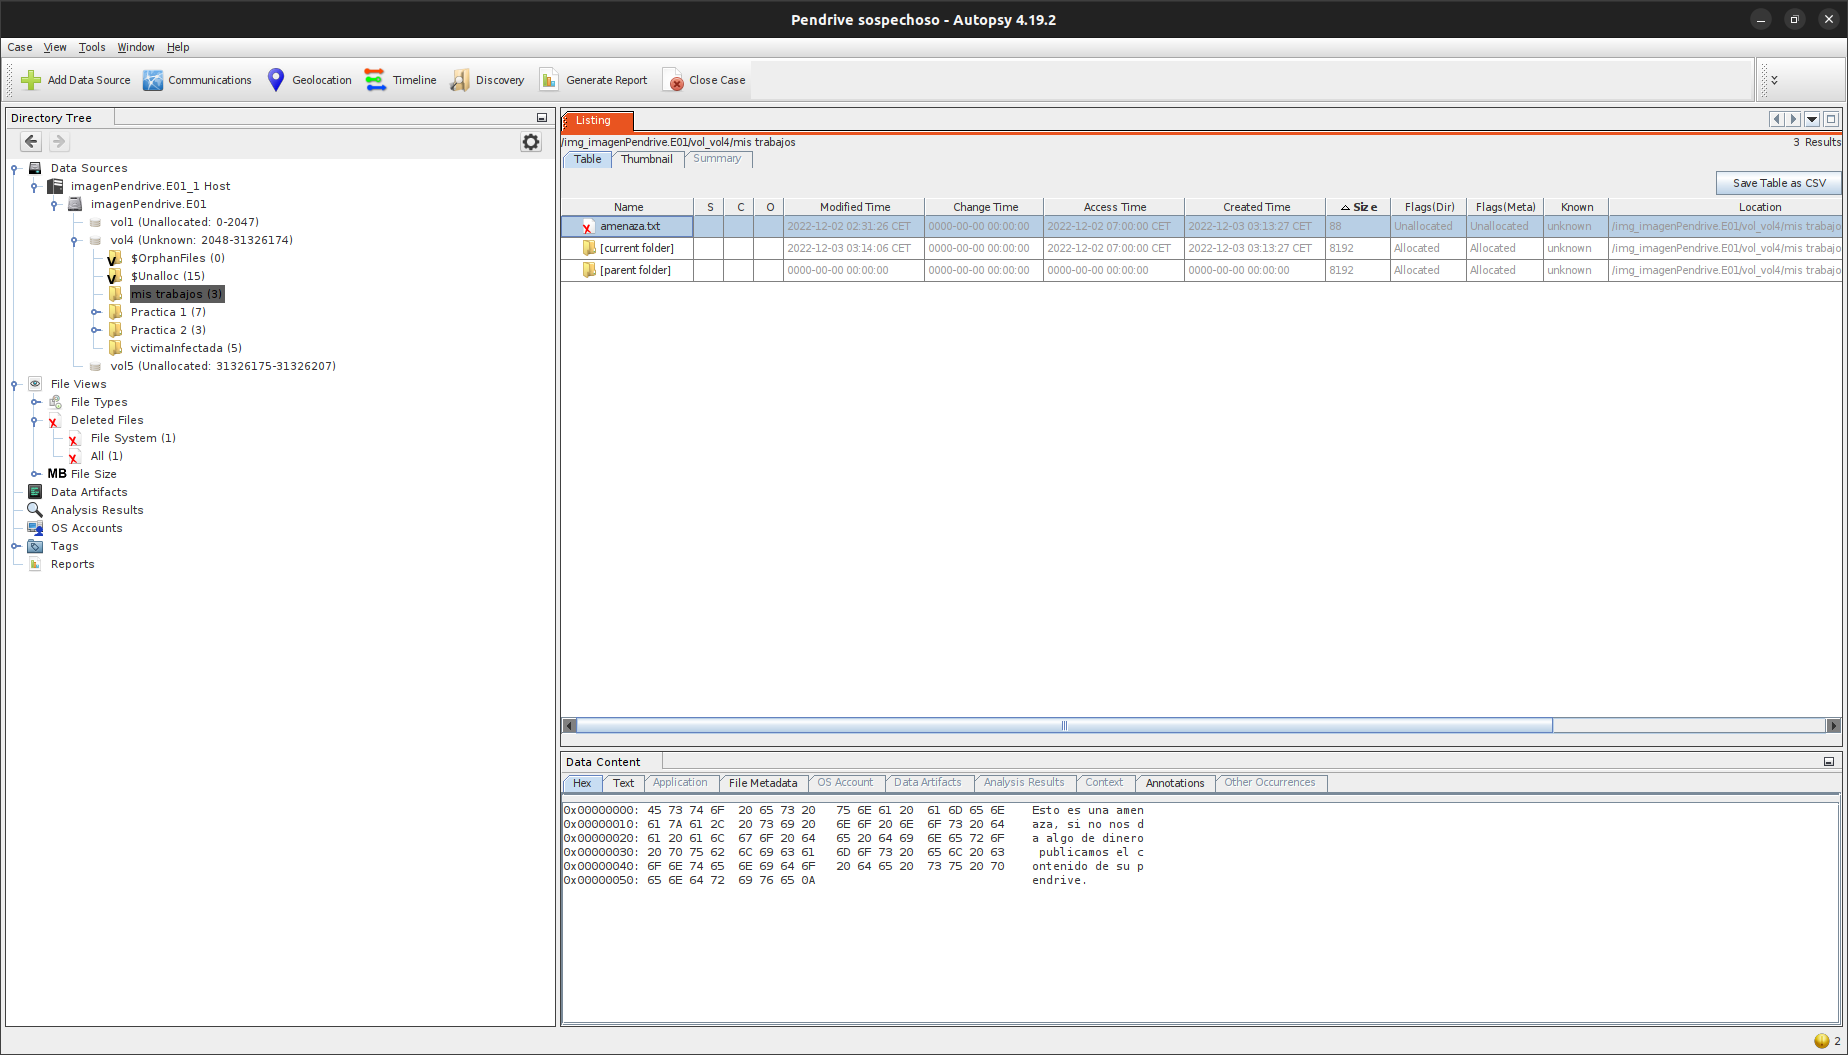
\includegraphics[width=\textwidth]{imagenes/Captura desde 2022-12-03 21-53-51.png}
    \caption{Archivo encontrado yendo a la ruta en el que se encontraba.}
\end{figure}

Y como se puede ver detecta el archivo eliminado del pendrive y muestra su información.

%SECCION DE IMAGENES DE WINDOWS

\phantomsection
\addcontentsline{toc}{subsection}{Apartado B}
\subsection*{Apartado B}

\textbf{NOTA: }Ahora voy a usar la versión de Windows de Autopsy, ya que me he dado cuenta de que contiene muchas más opciones que la versión de Linux no tiene (como ponerle nombre a las cuentas del sistema operativo, que en Linux no pasa, o poder ver los correos electrónicos).

\phantomsection
\addcontentsline{toc}{subsubsection}{a.- ¿Cuándo se creó la hoja de cálculo?}
\subsubsection*{a.- ¿Cuándo se creó la hoja de cálculo?}

Lo primero de todo es encontrar la hoja de cálculo en la imagen del ordenador de Jean. Es posible buscarla dándole a File Views $\rightarrow$ By Extension $\rightarrow$ Documents $\rightarrow$ Office.

%foto
\begin{figure}[H]
    \centering
    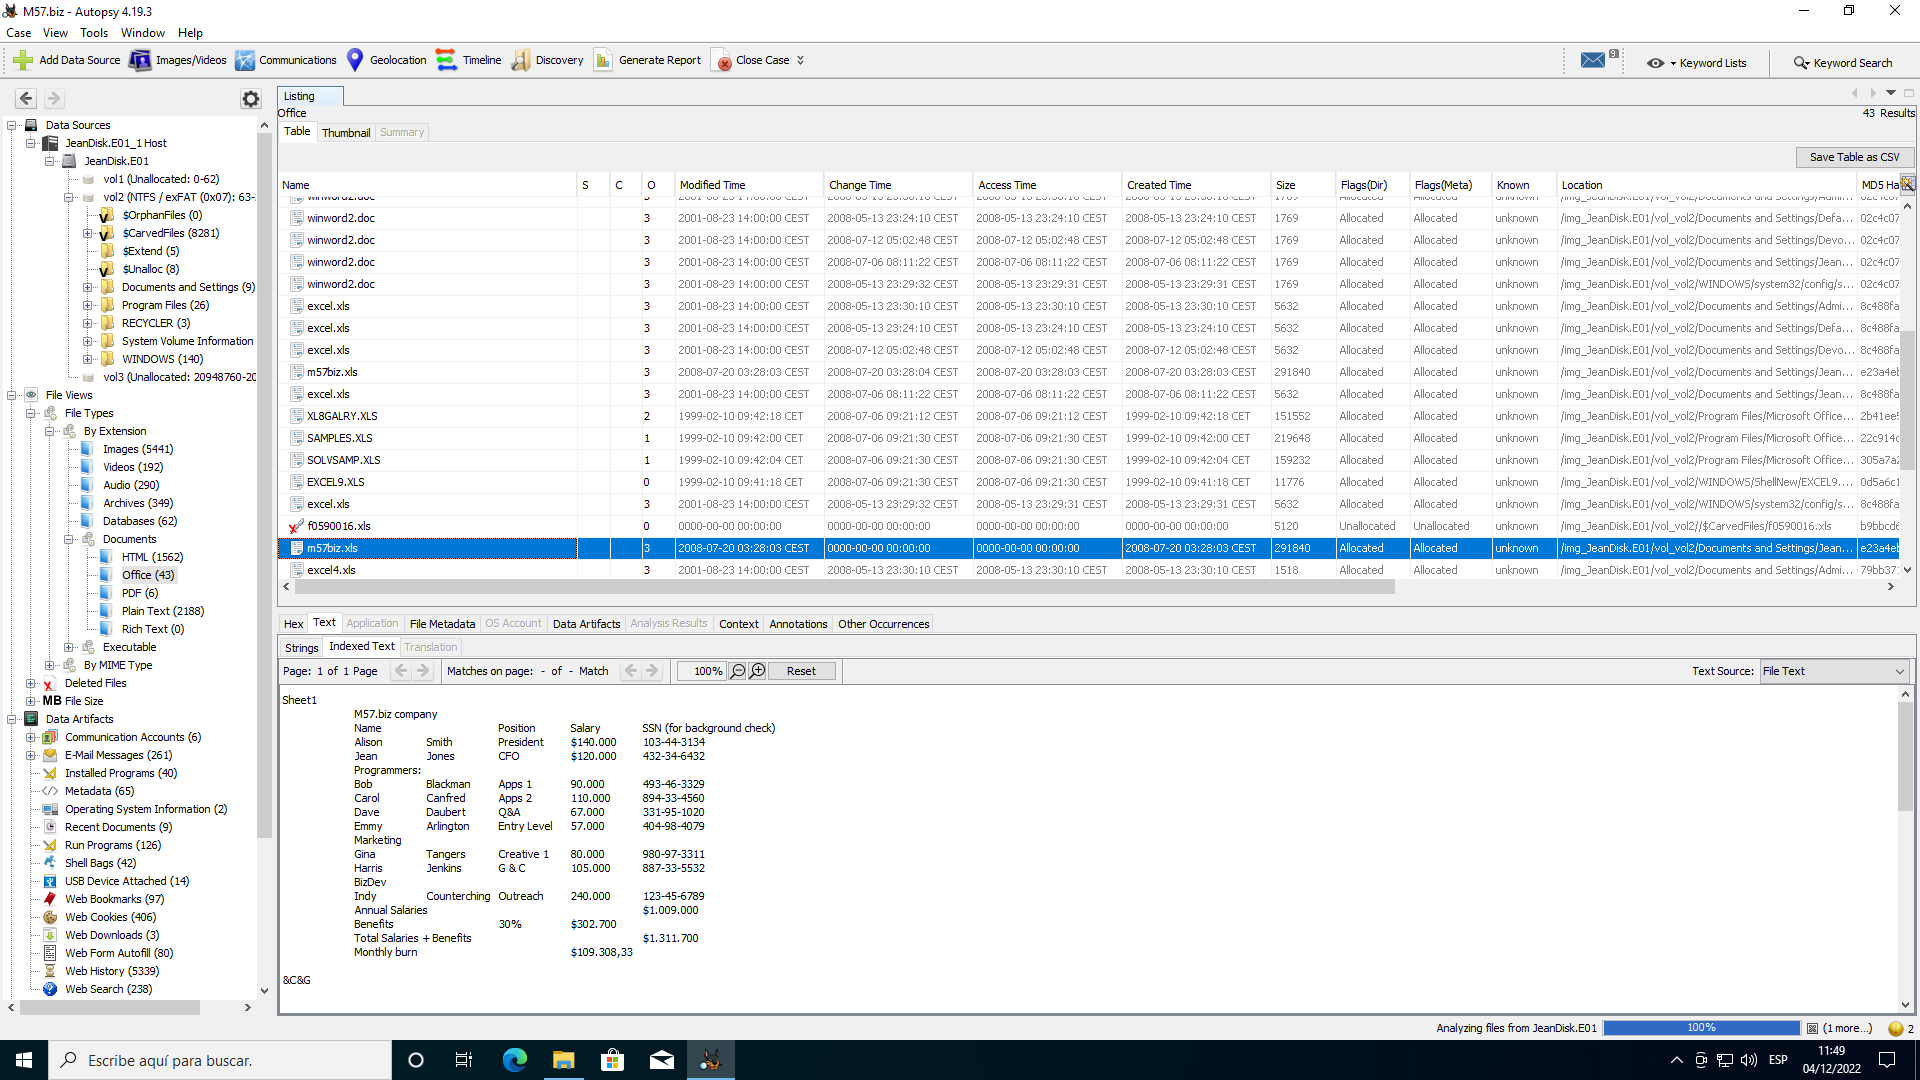
\includegraphics[width=\textwidth]{imagenes/Windows/Captura de pantalla (5).png}
    \caption{Como se puede observar abajo en ``Text'', es el documento que ha sido filtrado.}
\end{figure}

Ahora hay que darle a la pestaña ``File Metadata'' donde se indican todos los datos relacionados con el documento.

%foto
\begin{figure}[H]
    \centering
    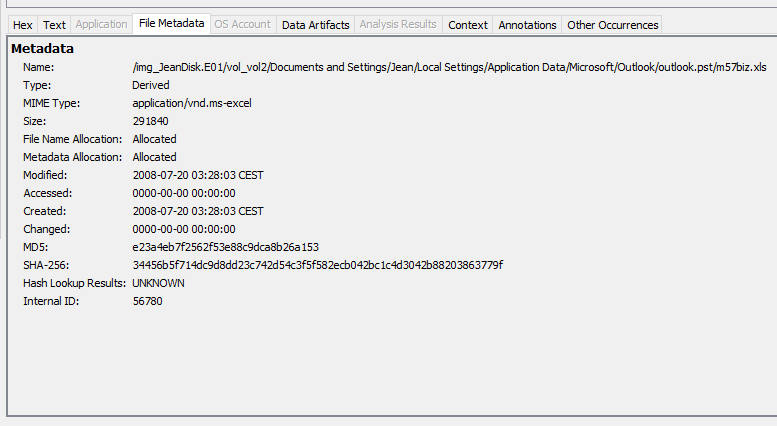
\includegraphics[width=\textwidth]{imagenes/Windows/Captura de pantalla (6).png}
    \caption{Metadatos de la hoja de cálculo.}
\end{figure}

Se puede ver que la hoja de cálculo fue creada el \textbf{20 de julio de 2008 a las 03:28:03 CEST}. Además, en la pestaña ``Text'', justo debajo del contenido del documento, aparecen más datos interesantes.

%foto
\begin{figure}[H]
    \centering
    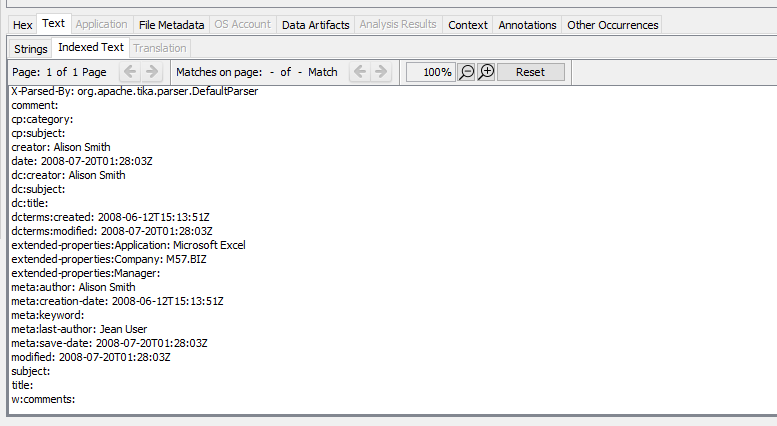
\includegraphics[width=\textwidth]{imagenes/Windows/Captura de pantalla (7).png}
    \caption{Más información sobre la hoja de cálculo.}
\end{figure}

El más notable es que fue creado por Alison Smith y que hay otra fecha de creación distinta a la pestaña de los metadatos, pero personalmente creo que es mejor fiarse de la de metadatos, ya que estos datos pueden ser modificados.

\newpage

\phantomsection
\addcontentsline{toc}{subsubsection}{b.- ¿Cómo llegó de su computador al sitio web de la competencia?}
\subsubsection*{b.- ¿Cómo llegó de su computador al sitio web de la competencia?}

Sabiendo los testimonios de los posibles implicados, se puede intuir que Jean envió por error la hoja de cálculo a otra persona, posiblemente a alguien de la empresa de la competencia.

\bigskip

Para tener pruebas fehacientes de esto, podemos mirar el historial de correos de Jean, para ello, nos vamos a Data Artifacts $\rightarrow$ E-Mail Messages $\rightarrow$ Default $\rightarrow$ Default.

%foto overview
\begin{figure}[H]
    \centering
    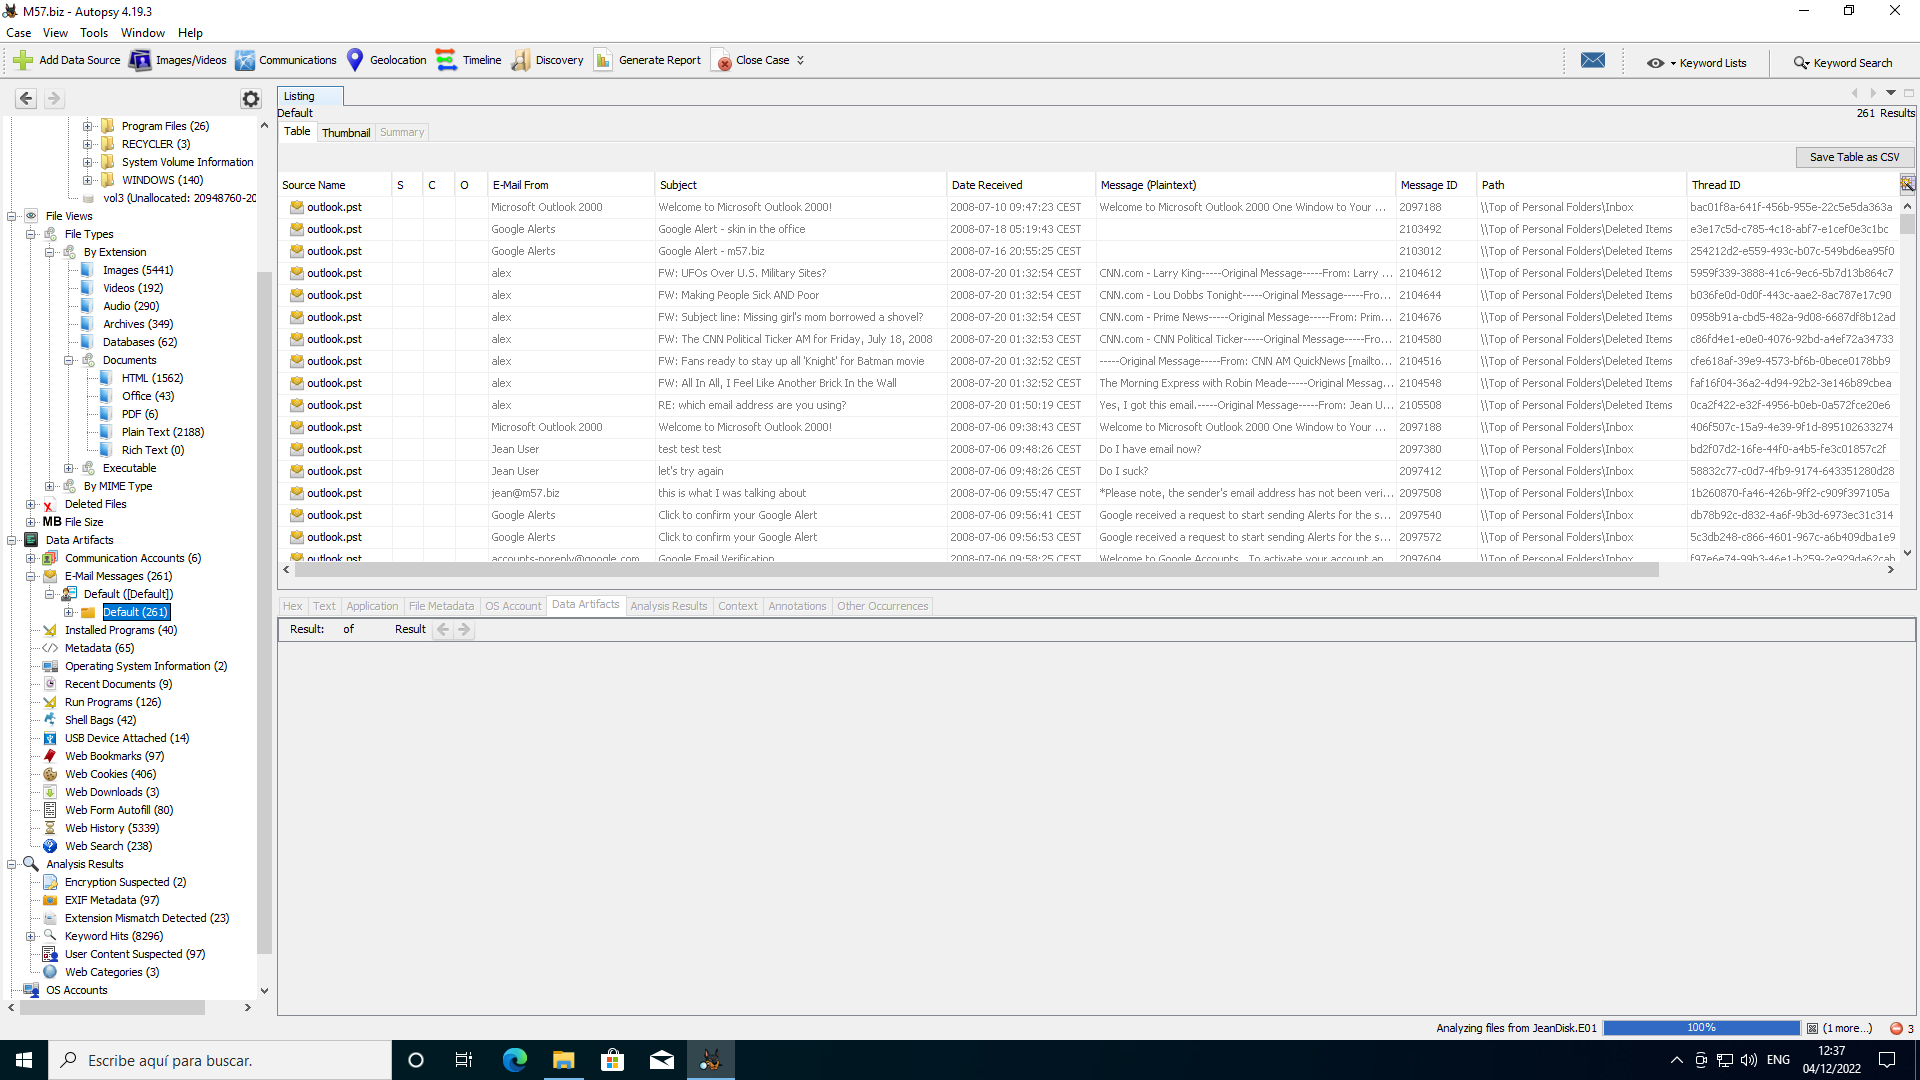
\includegraphics[width=\textwidth]{imagenes/Windows/Captura de pantalla (8).png}
    \caption{Correos recibidos y enviados en el ordenador de Jean.}
\end{figure}

Tras mirar la conversación entre Jean y Alison, pidiéndole a Jean que trabaje y que no mande correos extraños que parecen SPAM, aparece un correo muy interesante de Alison.

%fotos hacker
\begin{figure}[H]
    \centering
    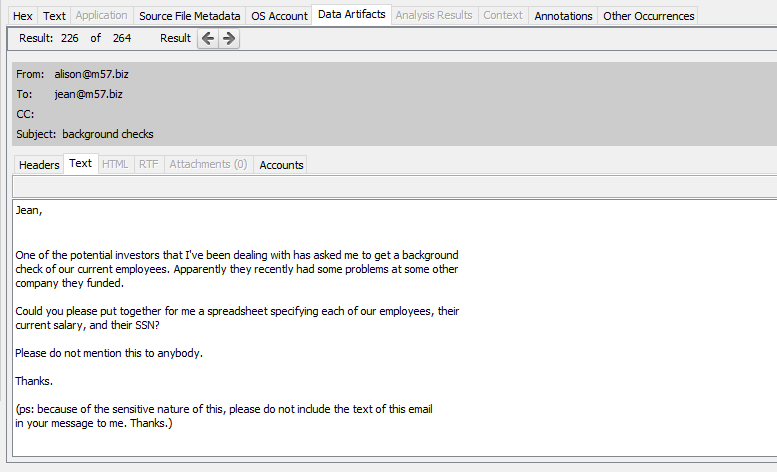
\includegraphics[width=\textwidth]{imagenes/Windows/Captura de pantalla (9).png}
    \caption{Alison, supuestamente, pidiéndole a Jean que le mande una hoja de cálculo con datos personales de los empleados.}
\end{figure}

\begin{figure}[H]
    \centering
    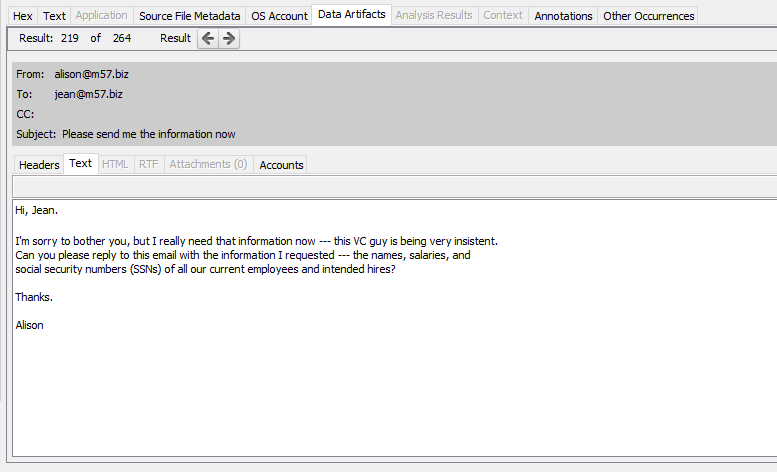
\includegraphics[width=\textwidth]{imagenes/Windows/Captura de pantalla (10).png}
    \caption{Se puede ver que le insiste a Jean que le envíe la información y le dice que no se lo diga a nadie.}
\end{figure}

Además, se ve que Jean le manda la hoja de cálculo que se ha filtrado y al día siguiente algunos empleados le preguntan que porque su información está en internet, preguntándole a Jean que si la que hay sobre él es correcta. Por tanto se puede asumir que el correo de Alison ha sido comprometido y ha sido usado de manera maliciosa para obtener estos datos.

%foto del attachment y mensaje
\begin{figure}[H]
    \centering
    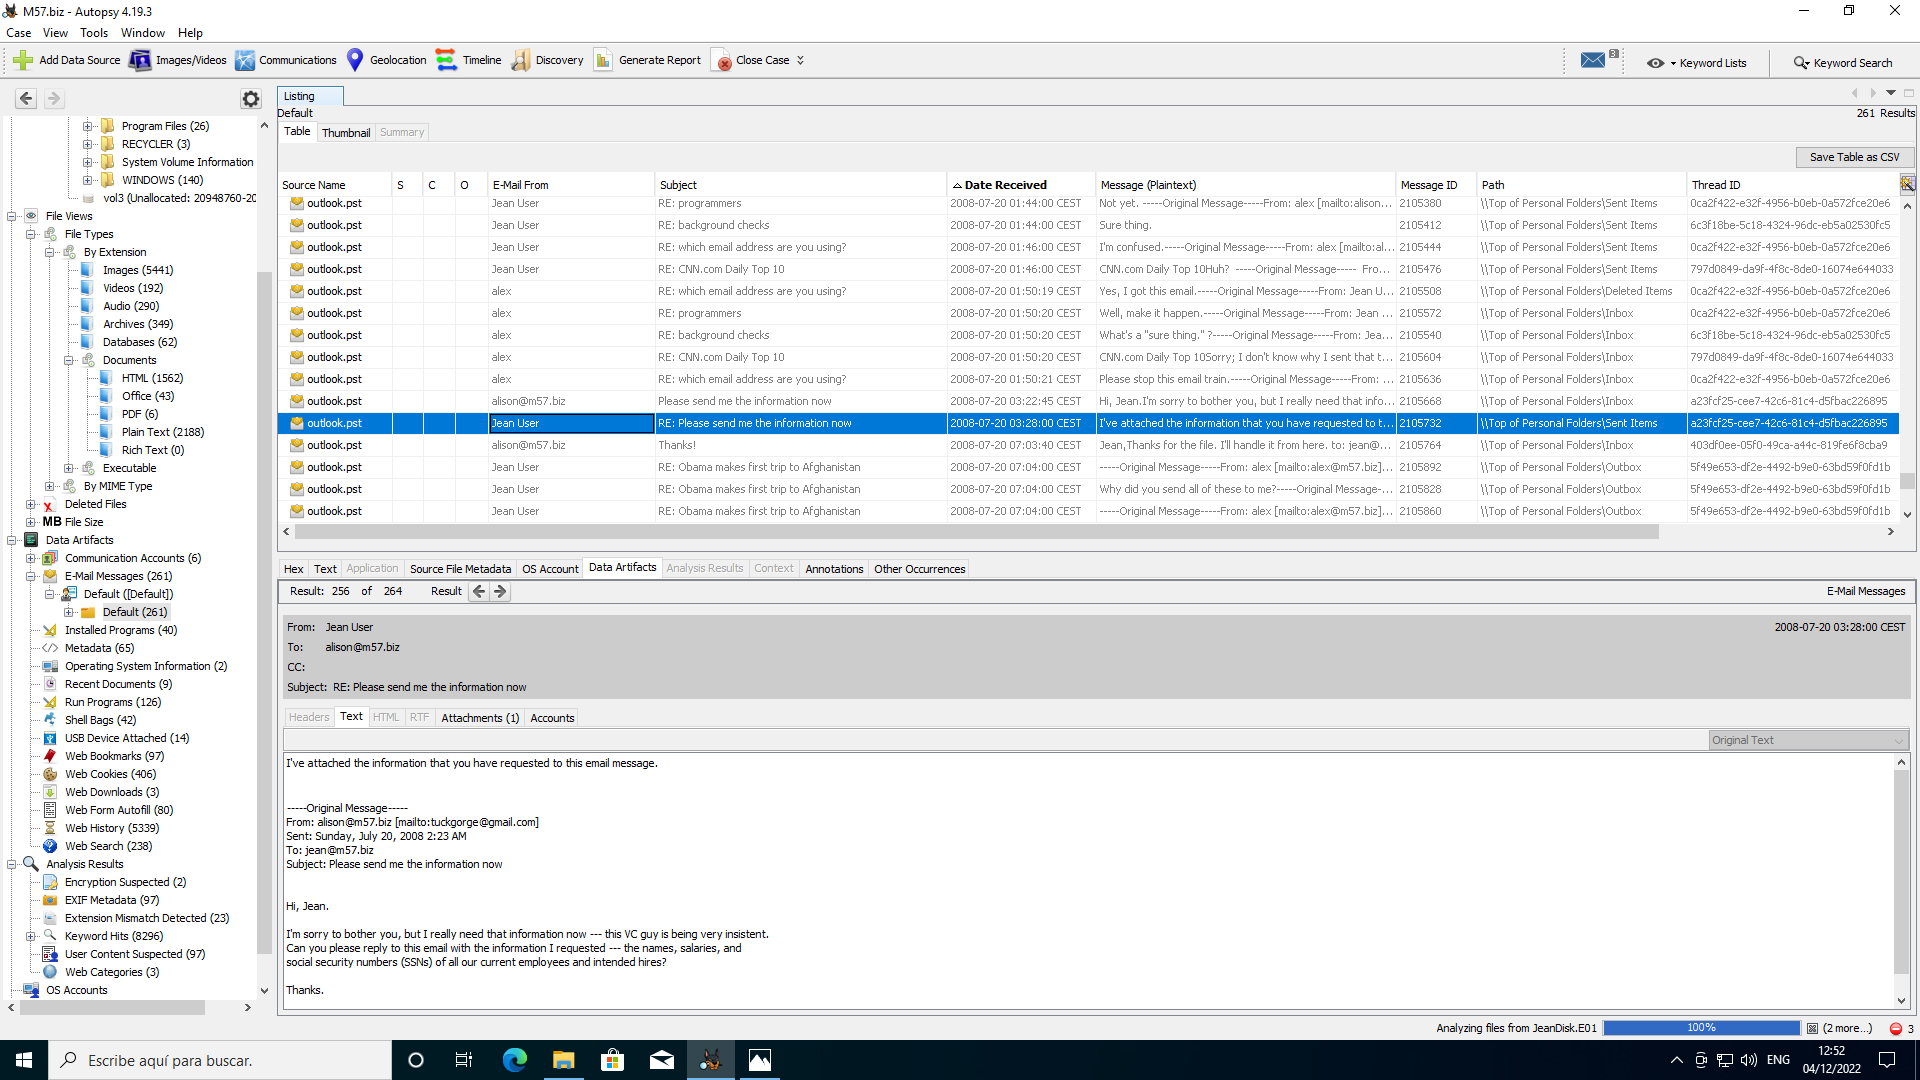
\includegraphics[width=\textwidth]{imagenes/Windows/Captura de pantalla (13).png}
    \caption{Mensaje que Jean le mandó con la hoja de cálculo.}
\end{figure}

\begin{figure}[H]
    \centering
    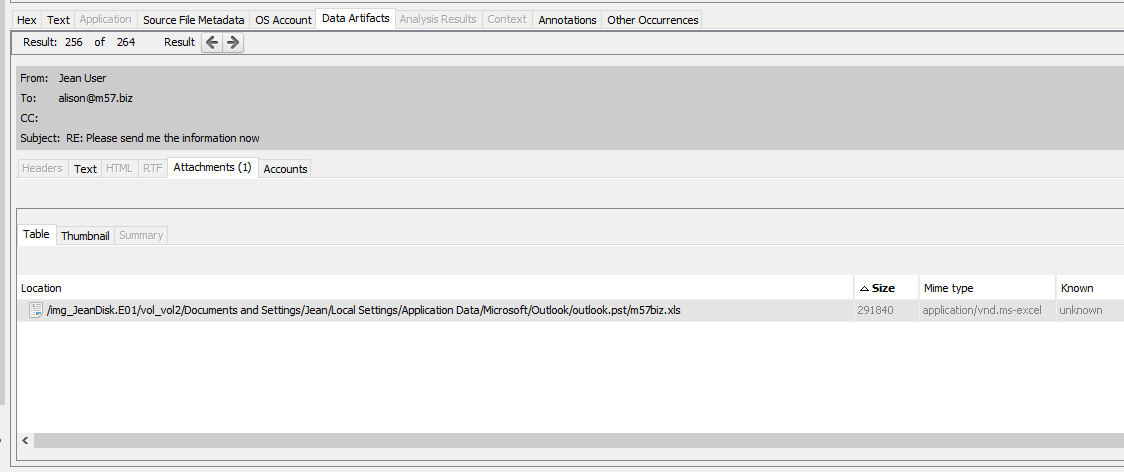
\includegraphics[width=\textwidth]{imagenes/Windows/Captura de pantalla (14).png}
    \caption{Hoja de cálculo adjunta en el correo.}
\end{figure}

%algunas fotos
\begin{figure}[H]
    \centering
    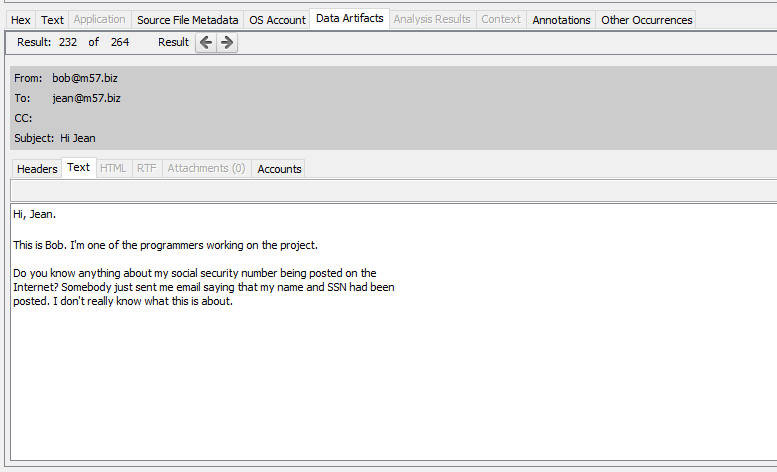
\includegraphics[width=\textwidth]{imagenes/Windows/Captura de pantalla (15).png}
    \caption{Un programador preguntando el motivo de la aparición de sus datos personales.}
\end{figure}

\begin{figure}[H]
    \centering
    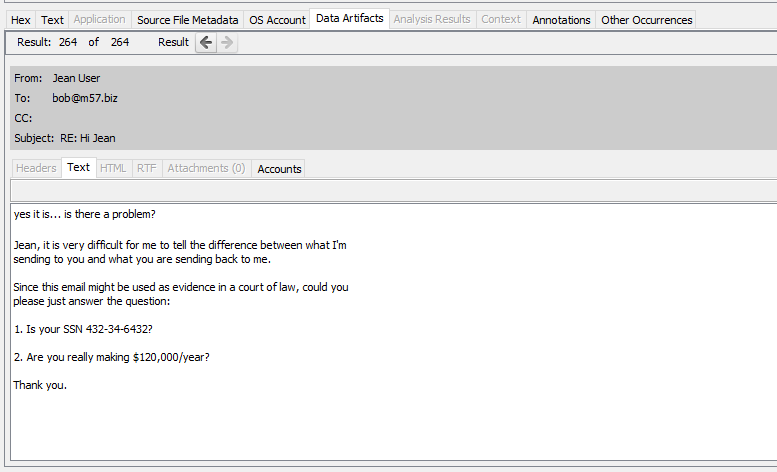
\includegraphics[width=\textwidth]{imagenes/Windows/Captura de pantalla (16).png}
    \caption{El propio Jean ha puesto sus datos también en la hoja de cálculo.}
\end{figure}

La conclusión final a esta pregunta es que Jean mandó al correo de Alison la hoja de cálculo, pero al estar mal configurado (de manera malintencionada o no) fue enviado al atacante.

\phantomsection
\addcontentsline{toc}{subsubsection}{c.- ¿Quién más de la compañía está involucrado?}
\subsubsection*{c.- ¿Quién más de la compañía está involucrado?}

Es difícil de saber, pero se sabe claramente que el correo de Alison tuvo un problema de configuración y estaba usando otra dirección de correo (alex@m57.biz) en el momento del ataque. Esto puede indicar que algún empleado obtuvo acceso al ordenador de Alison y ``desconfiguró'' su correo, dejando vía libre para poder usar el real. Puede que haya sido otro empleado descontento con la empresa que haya usado el correo de Alison para obtener la información, pero no se sabe a ciencia cierta.

\end{document}
